\documentclass[10pt,letterpaper,onecolumn]{article}
\usepackage[utf8]{inputenc}
\usepackage{geometry}
\geometry{
  letterpaper,
  total={170mm,257mm},
  left=20mm,
  right=20mm,
  top=20mm,
  bottom=20mm
}
\title{
  \textbf{ECE-GY 6473: COURSE PROJECT}\\
  \textbf{64-BIT MEMORY SYSTEM DESIGN}\\
  \textbf{New York University}\\ 
  \date{\textbf{Group 5:} Part 2 Submission - 12/10/18}
}
\author{
  I-Ting Chen\\
  \texttt{itc233@nyu.edu}
  \and
  Anurag Marwah\\
  \texttt{am8482@nyu.edu}
  \and
  Hard Patel\\
  \texttt{hap338nyu.edu}
  \and
  William Xia\\
  \texttt{wx312@nyu.edu}
}

\usepackage{tabu}
\usepackage{array}
\usepackage{natbib}
\usepackage{graphicx}
\usepackage{circuitikz}
\usepackage{xfrac}
\usepackage{amsmath}
\usepackage{subfig}

\begin{document}

\maketitle

\clearpage
\begin{center}
    This page is intentionally left blank.
\end{center}

\renewcommand*\contentsname{Table of Contents}
\clearpage
\tableofcontents

\clearpage
\title{\textbf{Table of Abbreviations:}}
\begin{table}[h!]
\centering
\begin{tabu} to 0.8\textwidth { | X[l] | X[l] | }
  \hline
  CLK & Clock \\ 
  \hline
  RE & Read Enable \\  
  \hline
  WE & Write Enable \\
  \hline
  WL & Word Line \\
  \hline
  BL & Bit Line \\
  \hline
  BL\_BAR & Bit Line Bar \\
  \hline
  PRE & Precharge \\
  \hline
  SA & Sense Amplifier \\
  \hline
  SAE & Sense Amplifier Enable \\
  \hline
  D & Data (Input of flip-flop) \\
  \hline
  SRAM & Static Random Access Memory \\
  \hline
\end{tabu}
\end{table}

\clearpage
\begin{center}
\section{SRAM Problem 1: Simulate Read and Write Operations}
\end{center}

\subsection{Schematic}
\begin{figure}[h!]
\centering
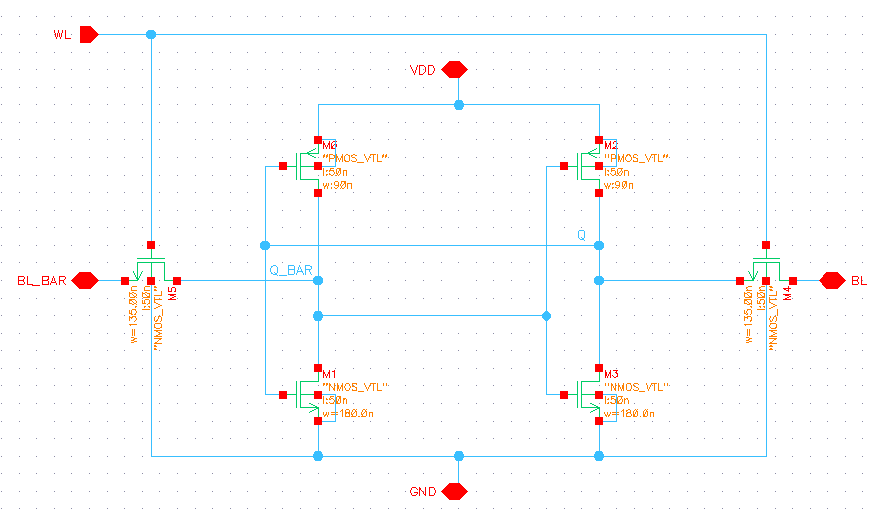
\includegraphics[clip,width=\columnwidth]{sram_cell_basic.png}
\caption{Basic SRAM Cell - Schematic}
\label{fig:sram_cell_basic}
\end{figure}

Figure~\ref{fig:sram_cell_basic} is the transistor level schematic of the 6-transistor SRAM cell used for memory system. Transistors M0, M1, M2, and M3 form cross-coupled inverters that hold the memory data in the nodes Q and Q\_BAR. The access transistors M4 and M5 connect the cell to the bit lines BL and BL\_BAR when the WL signal goes high.

\subsection{Waveforms}
\begin{figure}[h!]
\centering
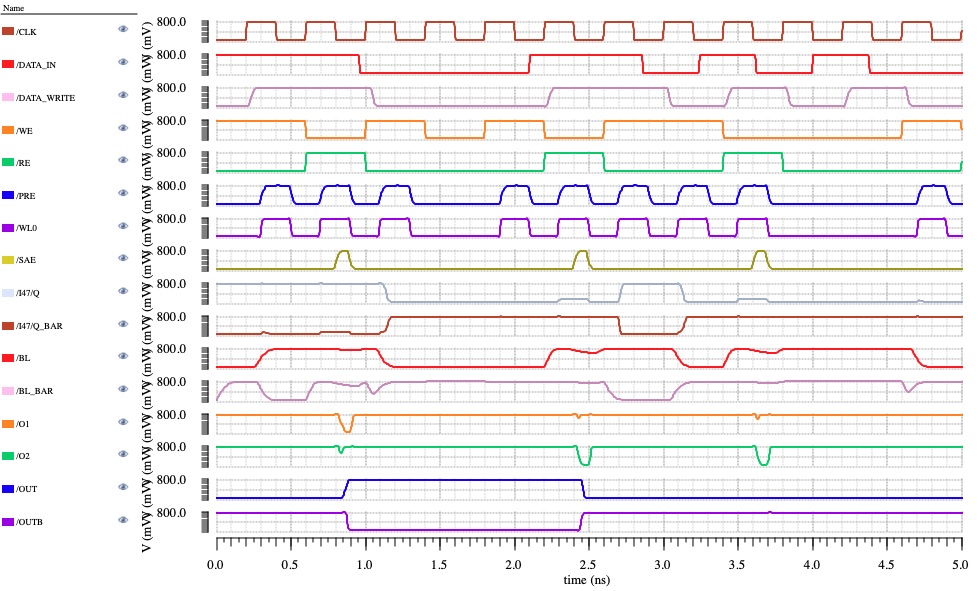
\includegraphics[clip,width=\columnwidth]{Problem1-TestRead-Write.png}
\caption{Read and Write Operations (Non-optimized Cell)}
\label{fig:Test_Read-Write}
\end{figure}

The waveforms shown in Figure~\ref{fig:Test_Read-Write} display the write and read operations to, and from the SRAM cell. In this section, we assumed the sizing of the SRAM cell to be the ratio $W_{Access}:W_{PullUp}:W_{PullDown} = 1.5:1:2$. The read and write operations function correctly on the SRAM cell.

\clearpage
\begin{center}
\section{SRAM Problem 2: Optimized Cell Transistor Design}
\end{center}

\subsection{Transistor Sizing: Design}

Designing the SRAM Cell required careful study of the width ratios between the access, pull-up, and pull-down transistors in the SRAM cell, as shown in Figure~\ref{fig:sram_cell_basic}. The sections below will discuss in depth the process for developing the optimal sizing. The required specifications are as follows:
\begin{itemize}
  \item Read Noise Margin: $>25\%$ of $V_{DD} = 187.5mV$
  \item Write Noise Margin: $>35\%$ of $V_{DD} = 262.5mV$
  \item SRAM Cell Area: $0.8\mu m^2$ (single cell)
\end{itemize}


\subsection{Parameters}

During the design process, it became clear that the area constraint would be the most difficult specification to meet. Thus, all subsequent sizing choices are made such that the area is be minimized, while still meeting the noise margins for the read and write operations. Please see Appendix A.3 for full tabulation of all experimental sizing used, and their respective noise margins.

\subsubsection{Read Margin}

The read noise margin depends on two important factors: the tripping voltage of the inverters in the cell, and the read voltage (or read disturb) that occurs when performing a read operation. Please see Appendix A.1 for the DC analysis used for testing and noise margin calculation.
\begin{figure}[h!]
\centering
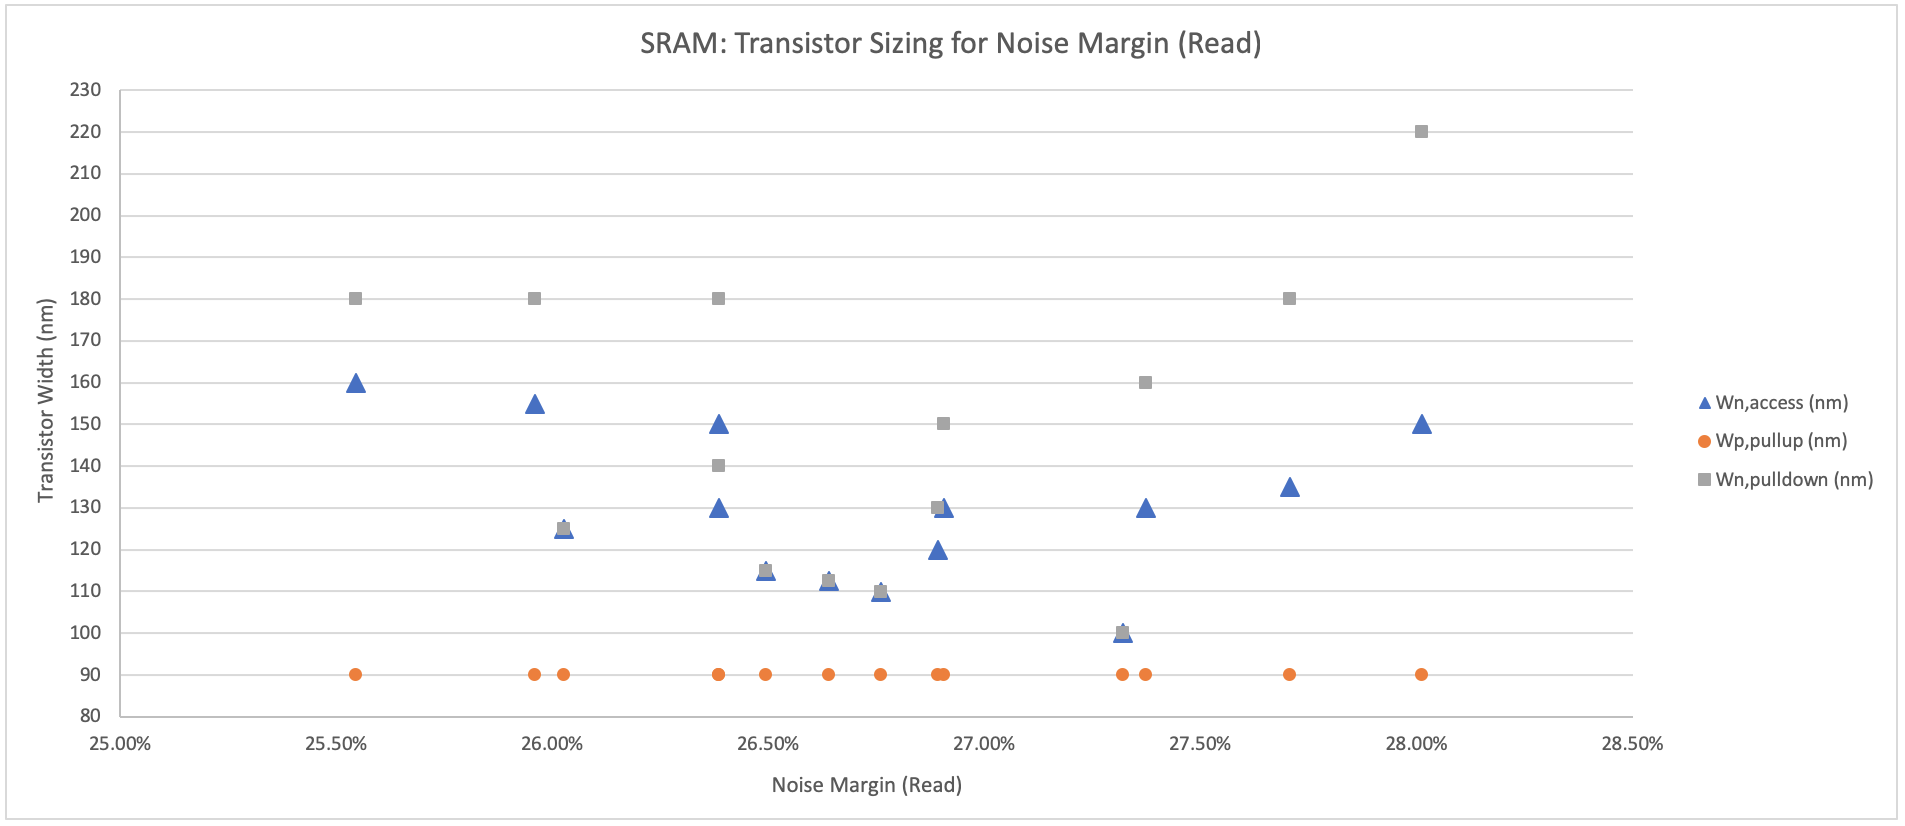
\includegraphics[clip,width=\columnwidth]{Problem2-NM_Read.png}
\caption{Transistor Sizing for Read Noise Margin}
\label{fig:NM_Read}
\end{figure}
Figure~\ref{fig:NM_Read} is a plot of the widths of all three transistors in the SRAM cell against the read margins found for each sizing. We can see that sizing the access and pull-down transistors the same width, and decreasing them can actually increase the read noise margin at smaller sizes. The behavior shown from sizing $W_{Access}:W_{PullUp}:W_{PullDown} = 110nm:90nm:110nm$ down to $100nm:90nm:100nm$ reflects this.
Since the read margin continues to be satisfied, even as we bring the transistor widths down to minimum size (90nm), we conclude that this specification is not the limiting factor. Thus, only analyzing the sizing relationship with the other constraints will provide the needed information for applicable design choices.

\subsubsection{Write Margin}
The write noise margin depends on the voltage levels in the bit lines during the write operation. The margin describes the largest error in the bit line voltage for which the SRAM cell can still register the correct data. Please see Appendix A.2 for the circuit and parametric analysis used for testing and noise margin calculation.
\begin{figure}[h!]
\centering
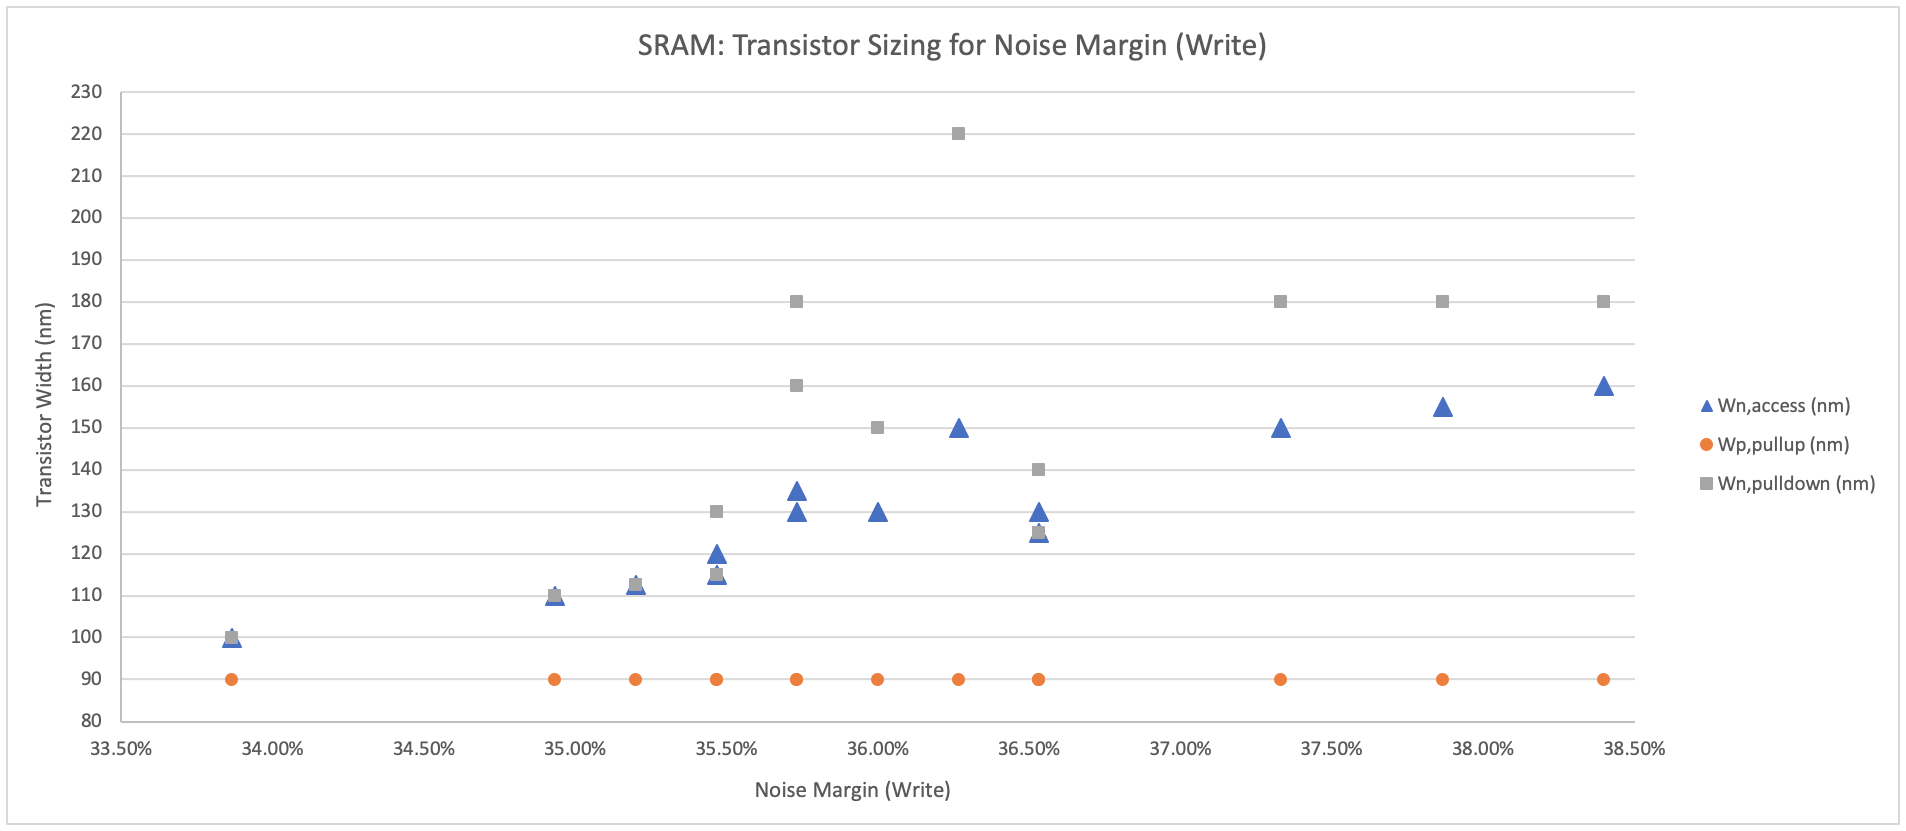
\includegraphics[clip,width=\columnwidth]{Problem2-NM_Write.png}
\caption{Transistor Sizing for Write Noise Margin}
\label{fig:NM_Write}
\end{figure}
Similarly as for the read margin, Figure~\ref{fig:NM_Write} is a plot of the widths of all three transistors in the SRAM cell against the write margins found for each sizing. It is clear that the write noise margin fails to meet specification once the access and pull-down transistor widths jointly reaches 110nm. As our prediction from studying the read margin suggests, the transistor sizing is indeed limited by the write margin.
We take the smallest possible ratio from Figure~\ref{fig:NM_Write} ($W_{Access}:W_{PullUp}:W_{PullDown} = 112.5nm:90nm:112.5nm$) and use this ratio for the SRAM design.

\subsubsection{Access Time}
\begin{figure}[h!]
\centering
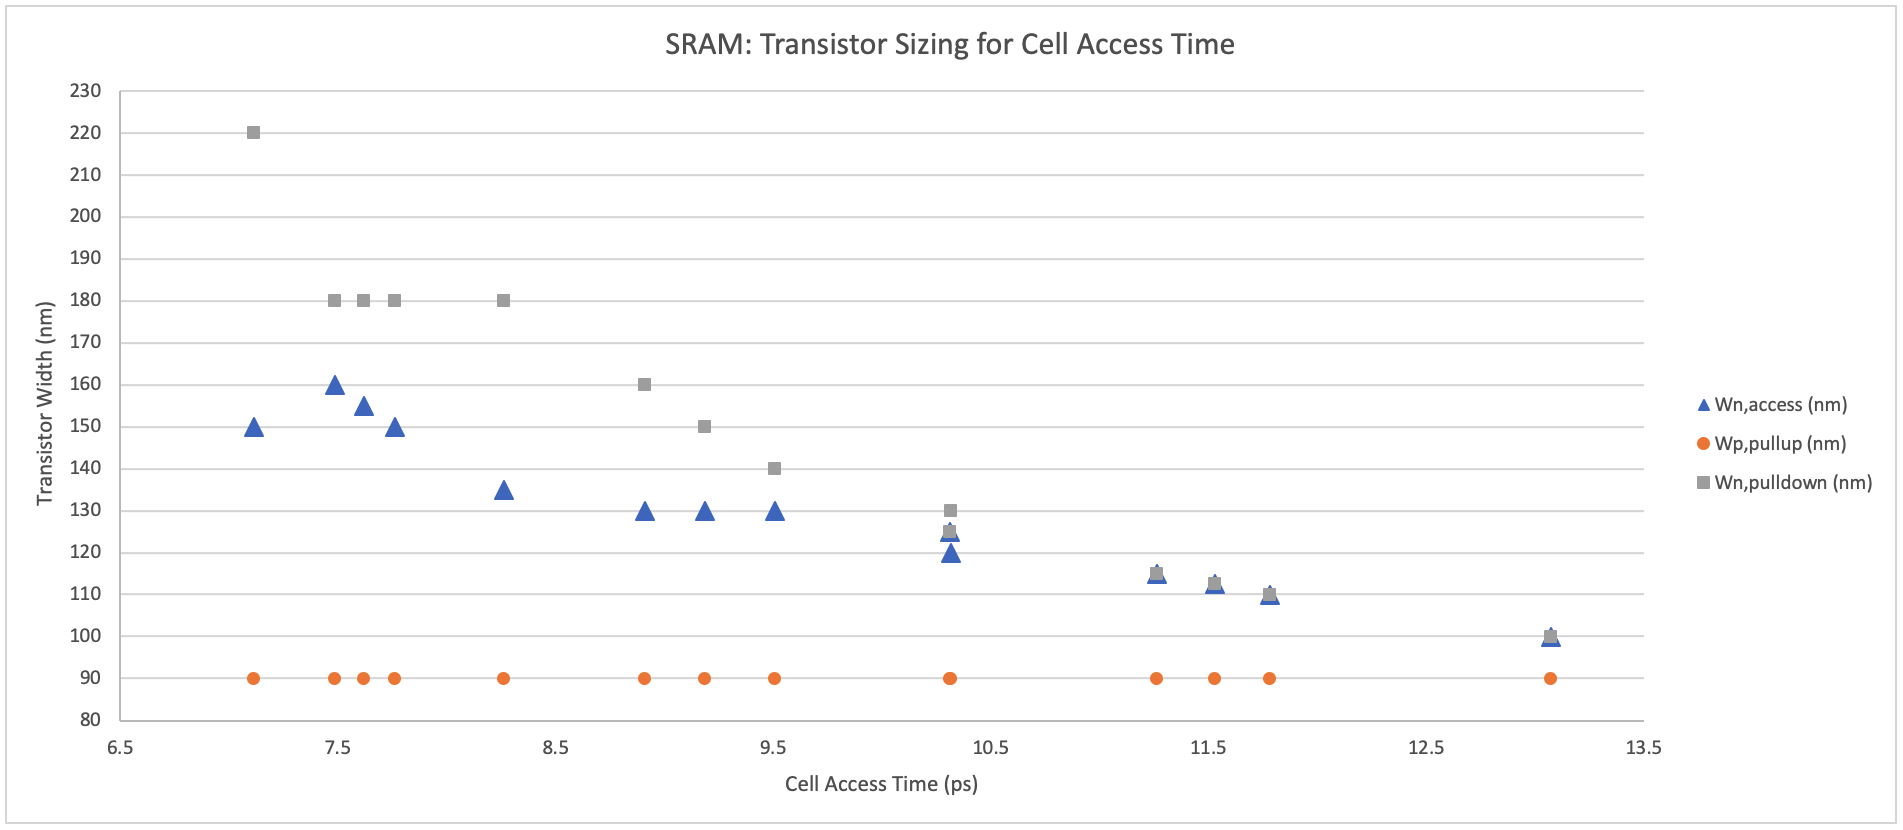
\includegraphics[clip,width=\columnwidth]{Problem2-CellAccessTime.png}
\caption{Transistor Sizing for Cell Access Time}
\label{fig:Cell_Access}
\end{figure}
The cell access time has been estimated for all the transistor ratios tested using the formula:
\begin{center}
    $T_{Access} = \frac{C_{bit}\times \Delta V_{bit}}{I_{read}}$
\end{center}
Where $C_{bit} = 40fF$ is the assumed bit line capacitance, $V_{bit} = 13mV$ is the sensitivity of our sense amplifer, and $I_{read}$ is the DC current that flows through the access and pull-down transistors during a read operation.\\
Please see Appendix A.1 the for analysis used to determine $I_{read}$. The results for all width ratios tested are shown in Figure~\ref{fig:Cell_Access}. These trends are expected since smaller transistor sizing increases the amount of time that is needed to access the cell. Note, that this is again not the limiting factor of the circuit.

\subsubsection{Cell Area}
To calculate the area of the SRAM cell, a formula is devised as below. This formula is only valid for the layout that is designed for the SRAM cell.\\
\\
$Area = Length\times Width$\\
$Length = 2\times [Max \{ 2\times Max\{ W_{Acc},W_{pd}\},W|^{min}_{P-well}\} + 2\times Spacing|^{min}_{(N-well,P-well)}]+(Max \{ 2\times W_{pu},W|^{min}_{N-well} \} )$
$Width = 2\times Body\,Length\,of\,Mosfet - Overlap\,Length = (2\times 370)-(30) = 710 nm$

\begin{table}[h!]
\centering
\begin{tabular}{ |l|l| }
  \hline
  \textbf{Variable} & \textbf{Description} \\ 
  \hline
  $W_{Acc}$ & Width of Access Transistor \\  
  \hline
  $W_{pd}$ & Width of Pull-down Transistor\\
  \hline
  $W_{pu}$ & Width of Pull-up Transistor \\
  \hline
  $W|^{min}_{P-well}$ & Minimum Width of P-well (=200nm) \\
  \hline
  $W|^{min}_{N-well}$ & Minimum Width of N-well (=200nm)\\  
  \hline
  $Spacing|^{min}_{(N-well,P-well)}$ & Minimum Spacing between N-well and P-well (=225 nm)\\
  \hline
\end{tabular}
\caption{Variables for Cell Area Formula}
\label{table:area_formula}
\end{table}

\subsection{SRAM Cell Design Summary}
The final sizing chosen for the SRAM cell was $W_{Access}$ = 112.5nm, $W_{PullDown}$ = 90nm, and $W_{PullUp}$ = 112.5nm. The resulting specifications for our design choice are:
\begin{table}[h!]
\centering
\begin{tabu} to 0.5\textwidth { | X[l] | X[c] | }
  \hline
  \textbf{Specification} & \textbf{Value} \\ 
  \hline
  $NM_{read}$ & $26.64\%$ \\  
  \hline
  $NM_{write}$ & $35.20\%$ \\
  \hline
  Cell Access Time & 11.53ps \\
  \hline
  Area & $0.781\mu m^2$ \\
  \hline
\end{tabu}
\caption{SRAM Cell Specifications}
\label{table:SRAM_specs}
\end{table}
Please refer to section 3 for full area calculation details.
\clearpage

\begin{center}
\section{SRAM Problem 3: Optimized Cell Layout}
\end{center}

\subsection{Layout}
\begin{figure}[h!]
    \centering
    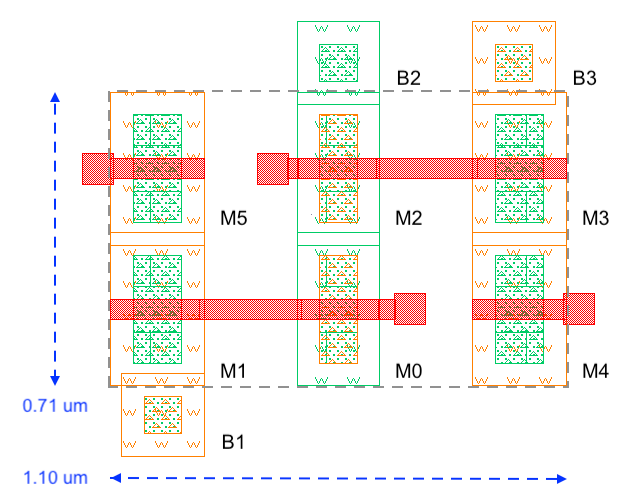
\includegraphics[clip,width=0.75\columnwidth]{sram_cell_placement.png}
    \caption{SRAM Cell - Placement}
    \label{fig:sram_cell_placement}
\end{figure}
Figure~\ref{fig:sram_cell_placement} shows the placement of the SRAM cell. M0 and M2 are the Pull-up Transistors, M1 and M3 are the Pull-down transistors, while M4 and M5 are the Access Transistors. B1, B2, and B3 are the body contacts to the P-well, N-well, and P-well respectively. The gates of the transistors are shown in red. M0 and M1 form one cross-coupled inverter, while M2 and M3 form the other cross-coupled inverter.
\begin{figure}[htp]
    \centering
    \subfloat[{Layout with Metal1 Layer}]{
    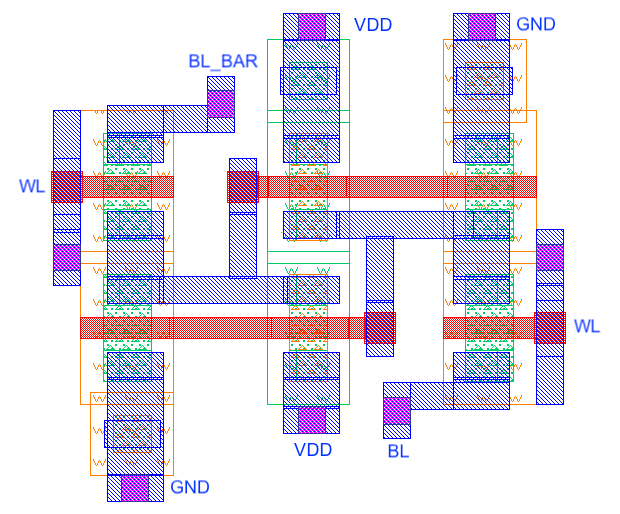
\includegraphics[clip,width=0.45\columnwidth]{sram_cell_layout_m1.png}
    }
    \subfloat[{Layout with Metal2 Layer}]{
    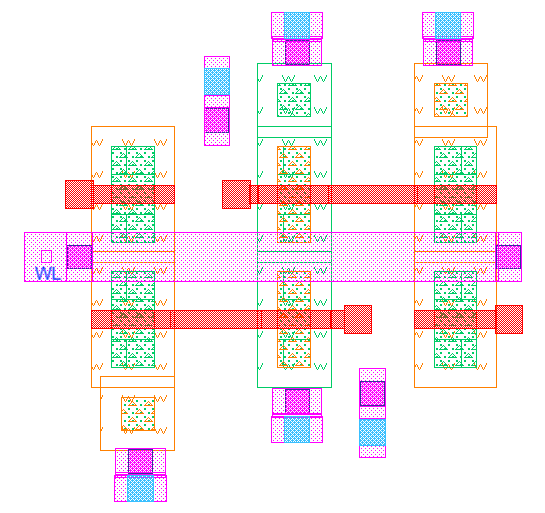
\includegraphics[clip,width=0.45\columnwidth]{sram_cell_layout_m2.png}
    }
    
    \subfloat[{Layout with Metal3 Layer}]{
    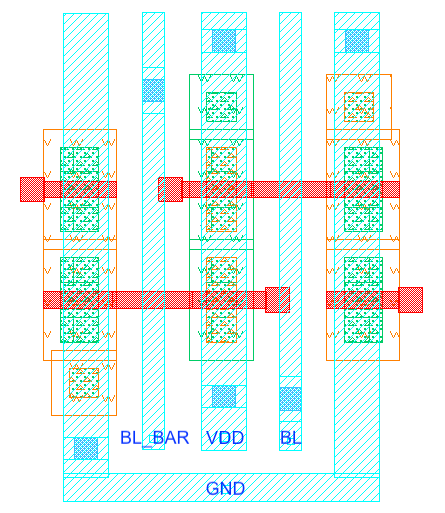
\includegraphics[clip,width=0.45\columnwidth]{sram_cell_layout_m3.png}
    }
    \subfloat[{Full Layout}]{
    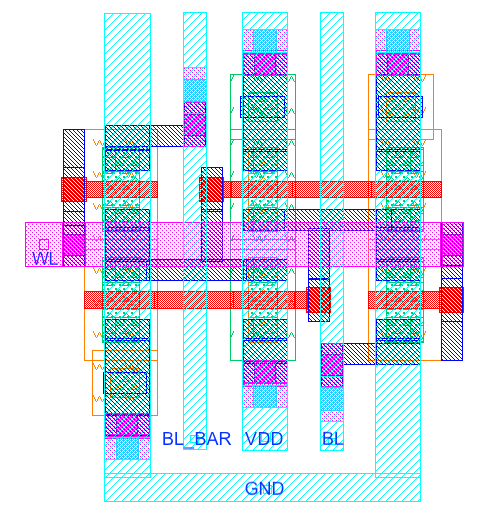
\includegraphics[clip,width=0.45\columnwidth]{sram_cell_layout_full.png}
    }
    \caption{SRAM Cell - Layout}
    \label{fig:sram_cell_layout}
\end{figure}
Figure~\ref{fig:sram_cell_layout} shows the complete layout of the SRAM cell, including higher metal layers. Part (a) shows the layout with Metal1 layer. Part (b) shows the layout with Metal2 layer. The WL signal is routed on the Metal2 layer. Part (c) shows the layout with Metal3 layer. The BL and BL\_BAR signals along with the VDD and GND power lines are routed on the Metal3 layer. Part (d) shows the complete layout with Metal1, Metal2, and Metal3 layers. 

\subsection{Area}
The area of the SRAM cell from edge-to-edge of the N-wells as calculated from Cadence is given below:
\begin{center}
$A = L\times W = 1.1 \mu m\times 0.71 \mu m = 0.781 \mu m^2$
\end{center}
The area of the SRAM cell including the body contacts and the vias to higher metal layers is given below:
\begin{center}
$A = L'\times W' = 1.325 \mu m \times 1.23 \mu m = 1.629 \mu m^2$ 
\end{center}
It is to note that the cell is repeatable on both the X and Y axes. So the effective area consumed per bit would be much lesser than $1.629 \mu m^2$. This is because of the lithography friendly design practice, like orienting all the transistors in the same direction, and not having a T-junction on the gate lines. These practices make the design physically more realizable. 
\subsection{DRC/LVS Report}
There are no DRC errors in the design and the LVS report is also correct. Figure~\ref{fig:DRC_Report} shows a summary of the DRC report. As indicated by the red boxes, there are no DRC errors in the design. Figure~\ref{fig:LVS_Report} shows a summary of the LVS report. As per the report, the design is LVS correct. Please see Appendix B for full DRC and LVS reports.\\
\begin{figure}[htp]
    \centering
    \subfloat[{DRC Results}]{
    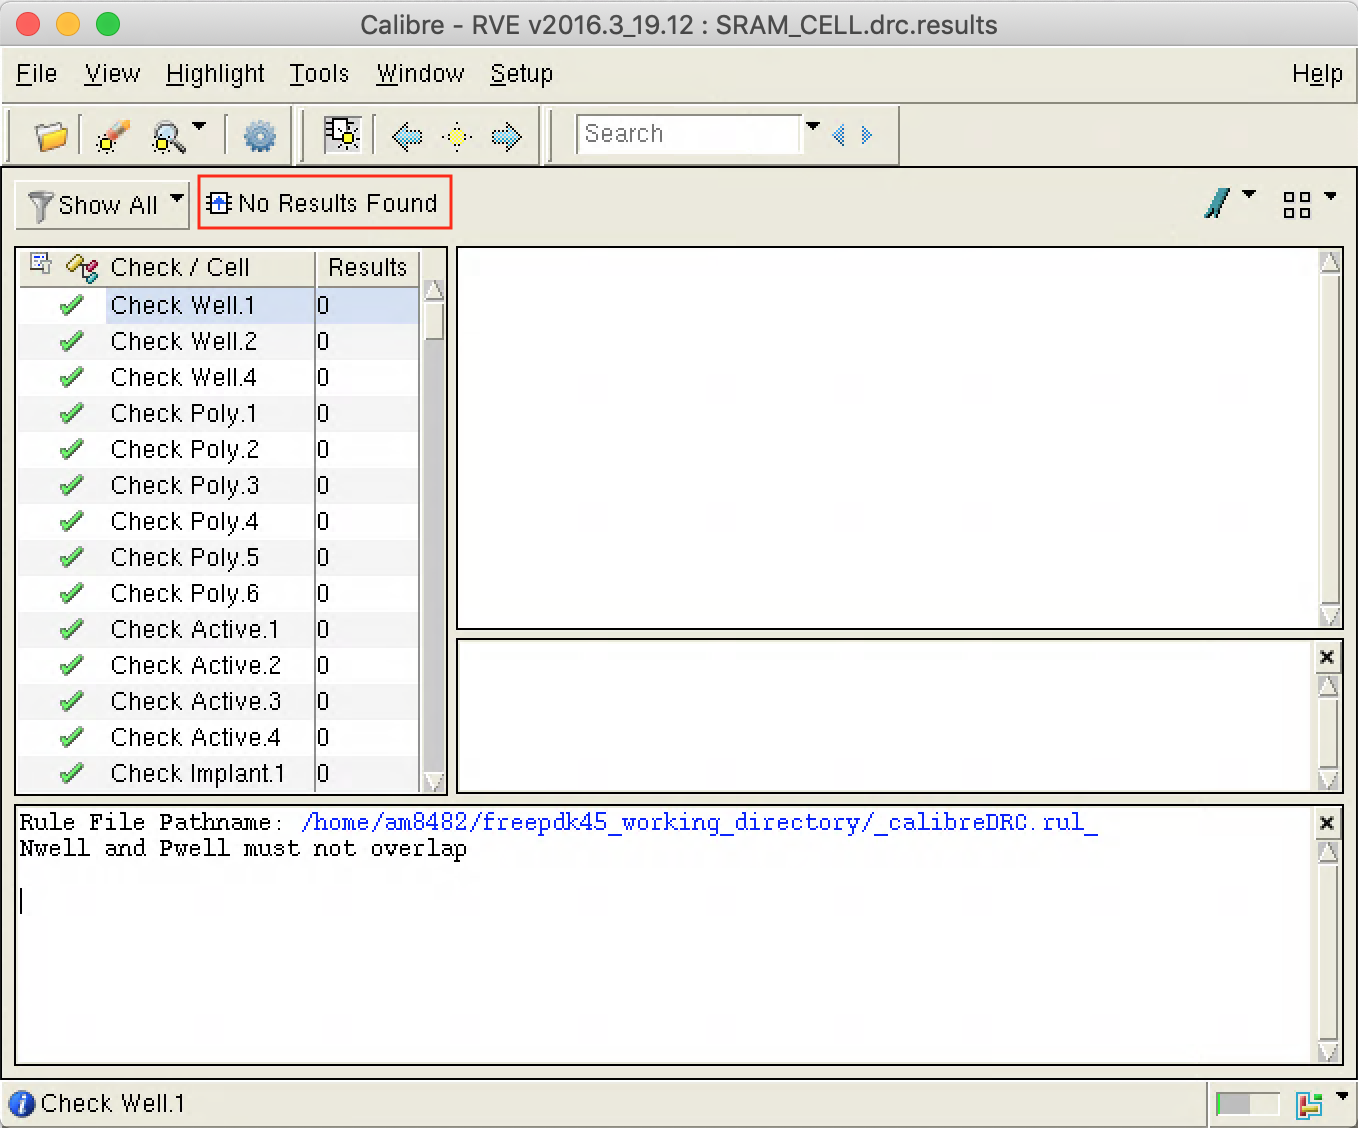
\includegraphics[clip,width=0.45\columnwidth]{DRC_Report_a.png}
    }
    \subfloat[{DRC Summary}]{
    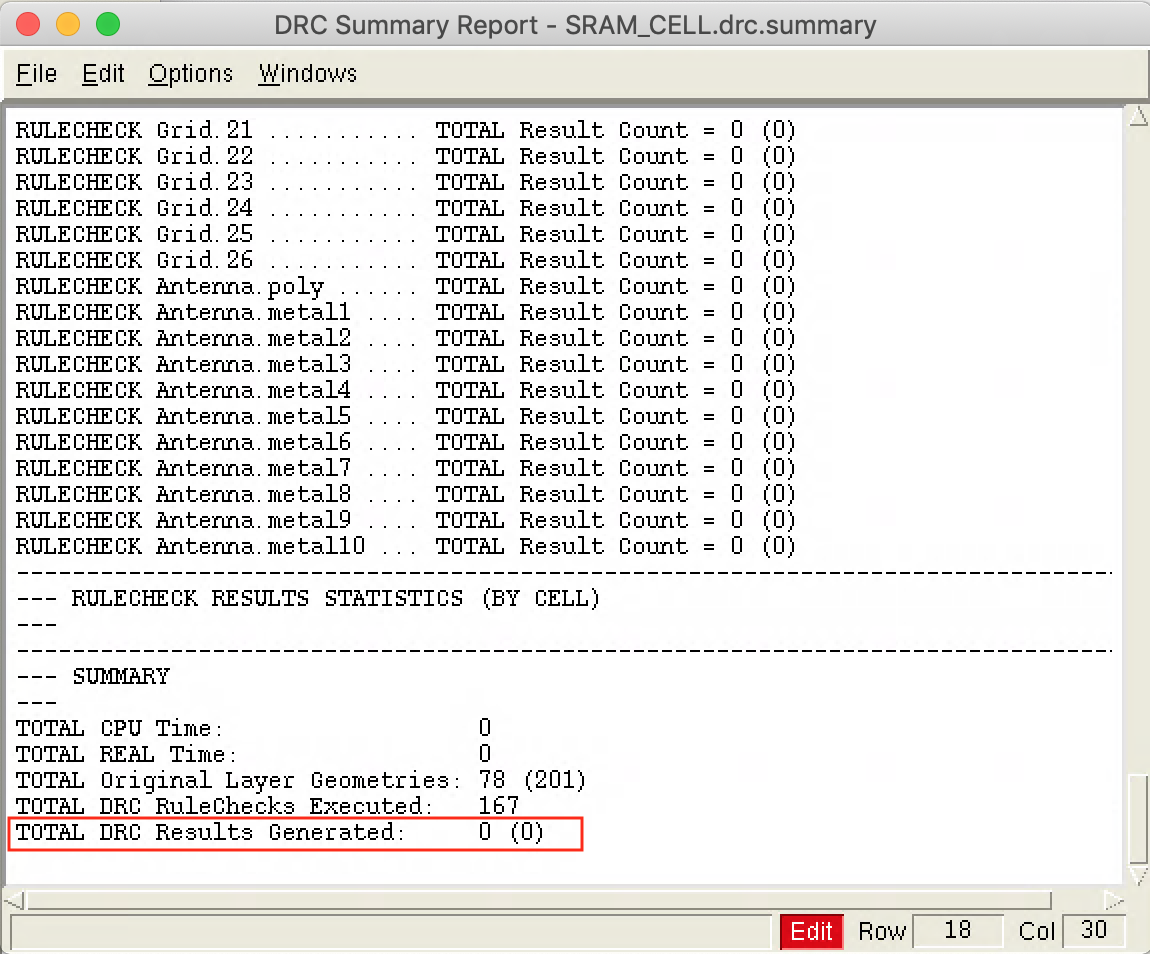
\includegraphics[clip,width=0.45\columnwidth]{DRC_Report_b.png}
    }
    \caption{SRAM Cell - DRC Report}
    \label{fig:DRC_Report}
\end{figure}

\begin{figure}[htp]
    \centering
    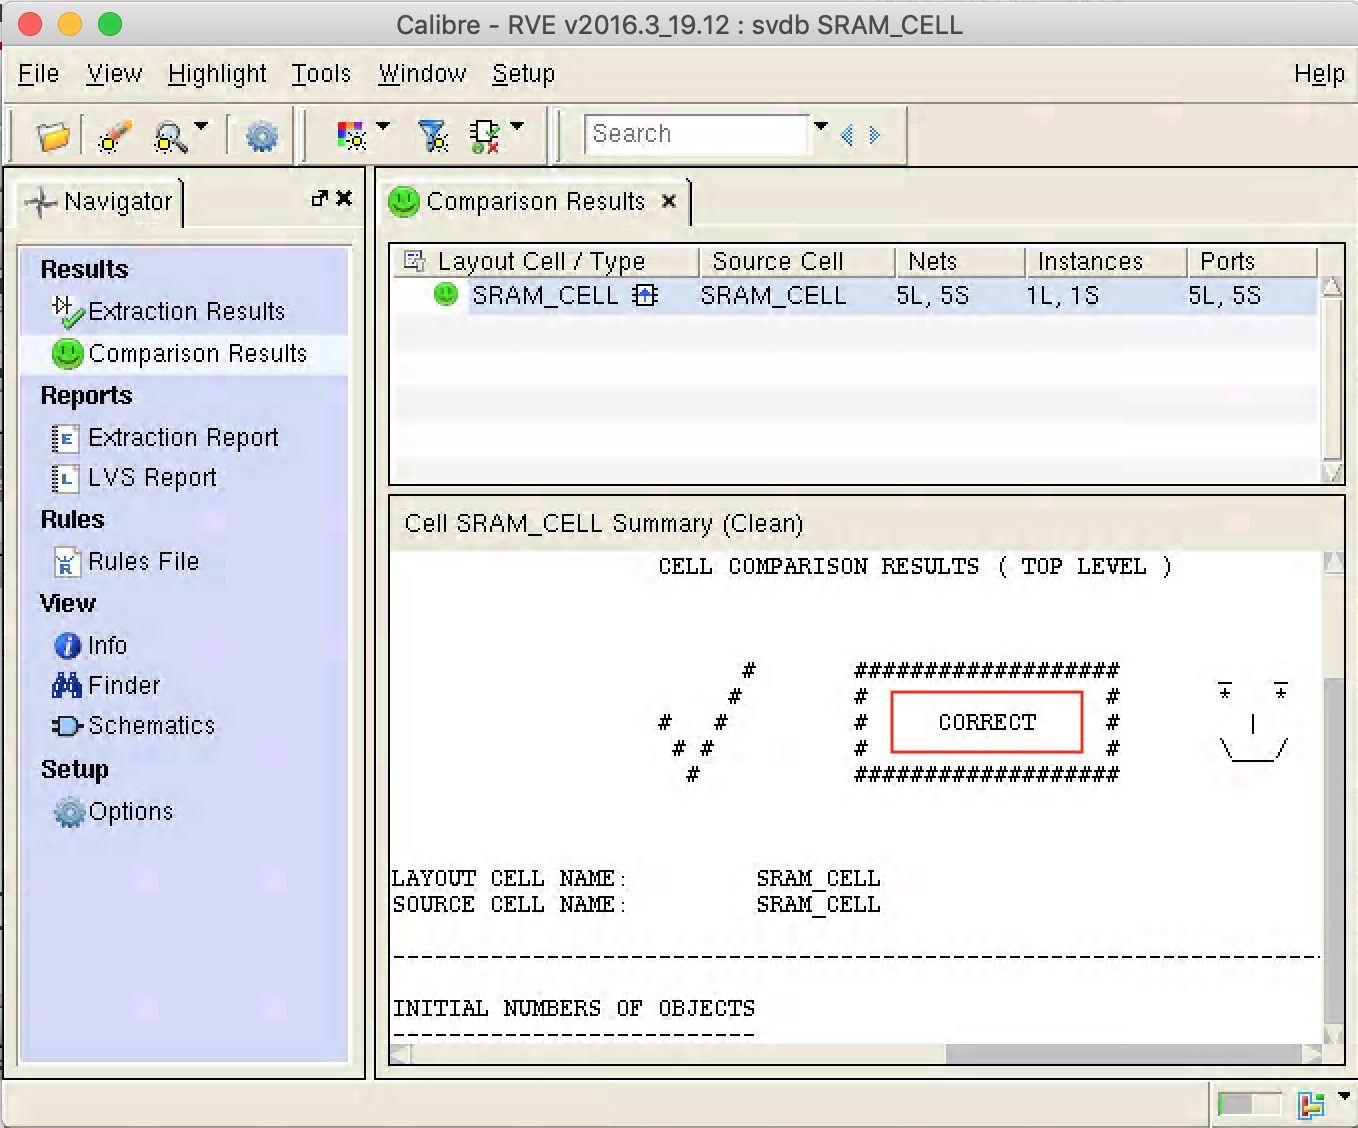
\includegraphics[clip,width=0.6\columnwidth]{LVS_Report.png}
    \caption{SRAM Cell - LVS Report}
    \label{fig:LVS_Report}
\end{figure}

\clearpage
\begin{center}
\section{SRAM Problem 4: Read and Write with Optimized Cell}
\end{center}
\subsection{Schematic}
\begin{figure}[h!]
\centering
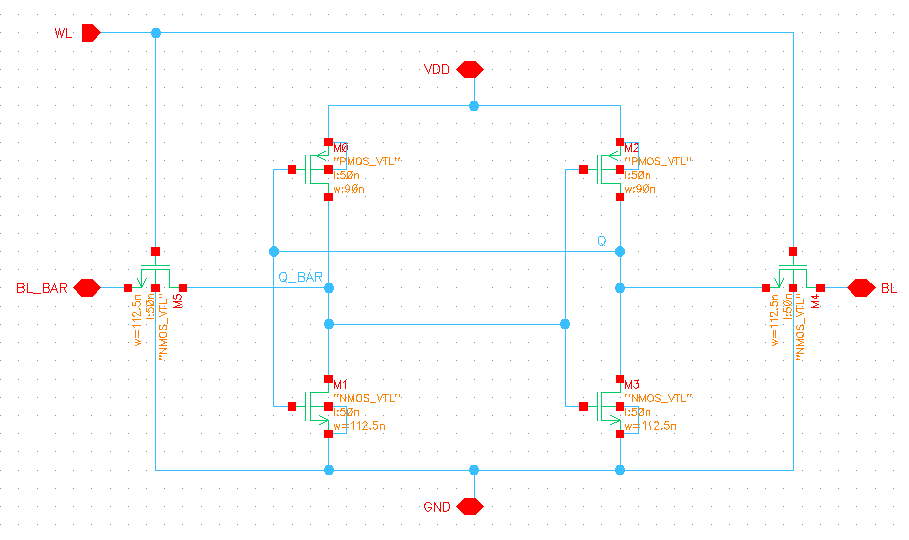
\includegraphics[clip,width=0.75\columnwidth]{sram_cell_schematic.png}
\caption{Optimized SRAM Cell - Schematic}
\label{fig:sram_sch_opt}
\end{figure}
\subsection{Waveform}
\begin{figure}[h!]
\centering
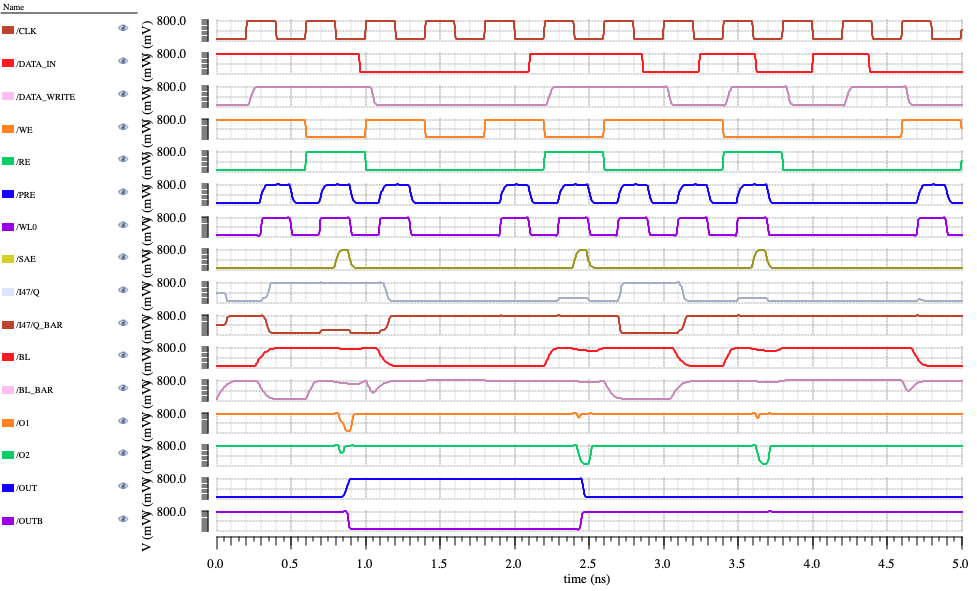
\includegraphics[clip,width=\columnwidth]{Problem4-TestRead-Write.png}
\caption{Read and Write Operations (Optimized Cell)}
\label{fig:Test_Read-Write_opt}
\end{figure}
Figure~\ref{fig:Test_Read-Write_opt} shows the read and write operation with the same parameters as those used for the simulation shown in Figure~\ref{fig:Test_Read-Write}. Comparing the two, we see that the read and write operations are performed correctly.
\subsection{Timing}
The final timing specifications for the circuit are as follows:
\begin{itemize}
  \item CLK to WL: $96.83ps$
  \item Cell Access Time: $11.53ps$
  \item Sense Amplifier: $38.18ps$
  \item SAE to Output of latch: $79.10ps$
\end{itemize}
Note that the delay from the rising edge of the clock to the rising edge of WL is approximately 100ps, as per our design. This will be further discussed in section 4.3.1. 
\subsubsection{Signal Generation}
\begin{figure}[h!]
\centering
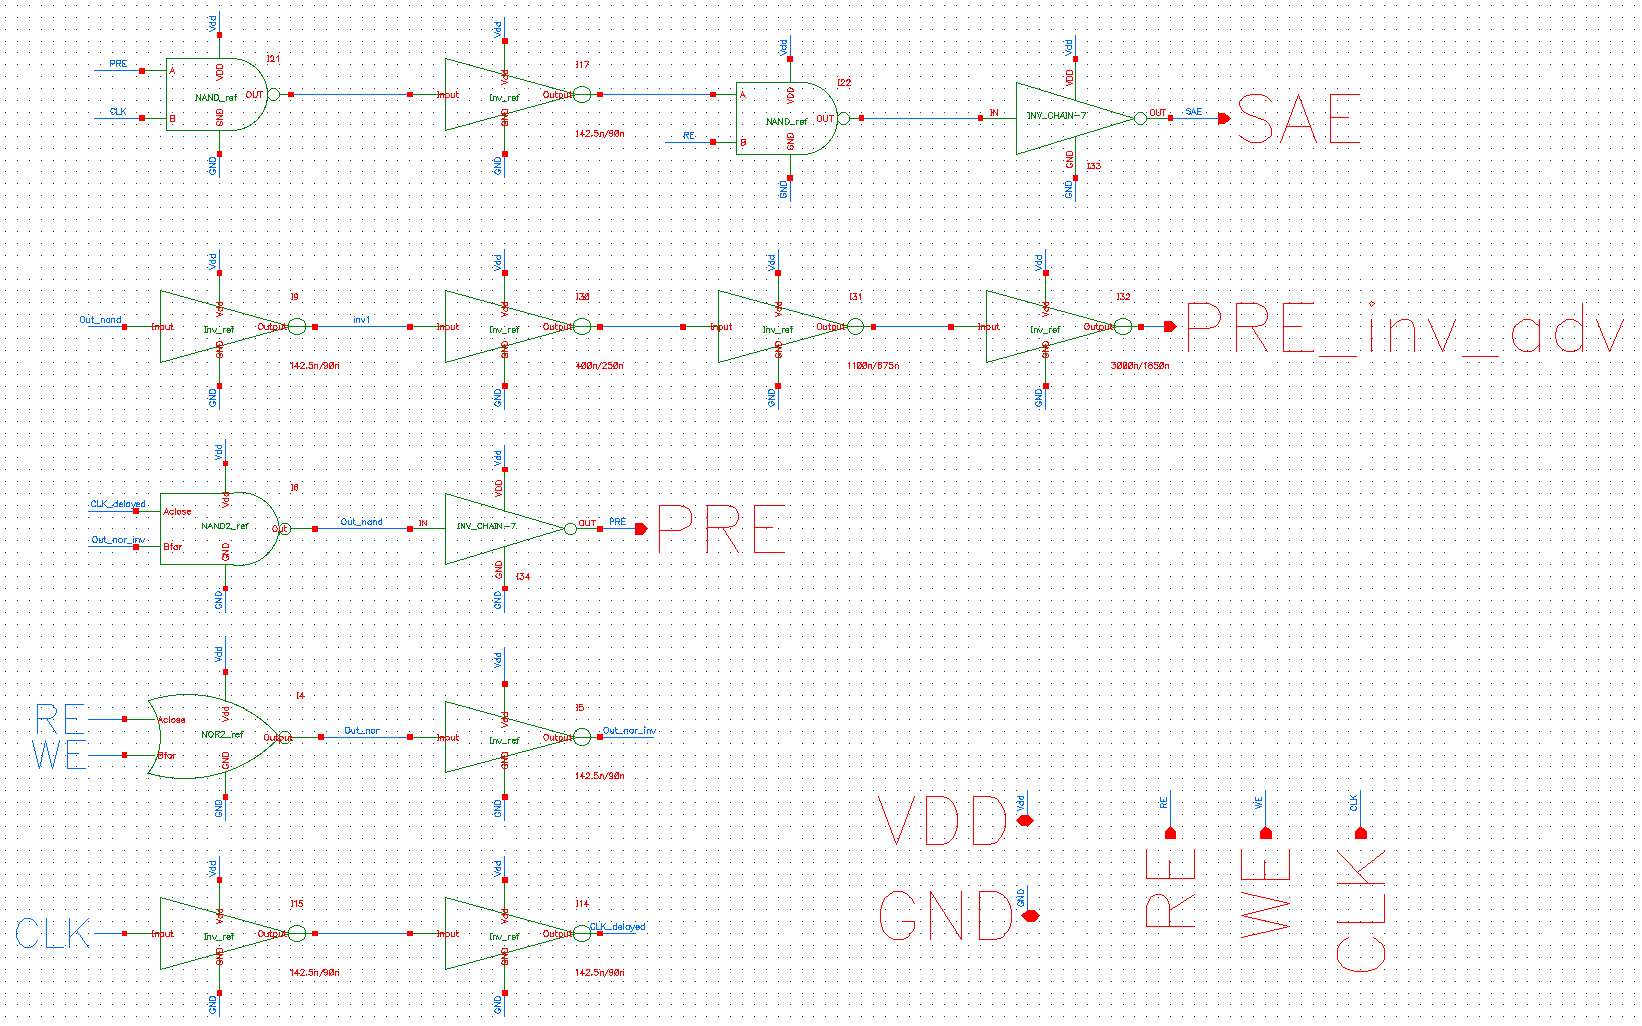
\includegraphics[clip,width=0.9\columnwidth]{SIGNAL_GEN.png}
\caption{Signal Generation - Schematic}
\label{fig:signal_gen}
\end{figure}
Figure~\ref{fig:signal_gen} shows the circuit used for generating the control signals SAE, PRE, and an additional signal PRE\_inv\_adv. The PRE and SAE signals are same waveforms that are shown in Figure~\ref{fig:Test_Read-Write_opt}. The PRE\_inv\_adv signal is the time advanced version of inverted PRE. It is used for synchronizing WL with the PRE. The time advancing is done to synchronize PRE \& WL to a greater extent. \\
PRE is a delayed version of clock which should be high only when memory is either reading or writing. That is, when $RE \cup WE = 1$. So basically, the signal generator implements below logic for PRE: 
\[
    PRE = CLK_{delayed}\cap (RE\cup WE)
\]
SAE signals should only be high when CLK is high, PRE is high, and RE is high. Thus, we use two NAND2 gates with inverters to generate the effective logic:
\[
    SAE = CLK\cap RE\cap PRE_{delayed}
\]
The delayed version of CLK and PRE are generated using inverter chains. PRE uses minimum sized inverter chain, whereas PRE\_inv\_adv uses progressively sized inverter chain due to the fact that it observes large gate capacitances when synchronizing with WL. 

\subsubsection{Maximum Frequency}
The maximum frequency the circuit can be operated (with the current design) is with a clock period of 350ps. This corresponds to a maximum clock frequency of 2.86GHz. Figure~\ref{fig:max_freq} shows the full peripheral performing correct read and write operations to a single SRAM cell. Note that as the clock frequency is increased, the pulse width of the SAE signal is effectively decreased. This is due to our design choice to delay the SAE rising edge by 100ps after the rise of the WL. This choice serves to conserve power in the sense amplifier during each read cycle.

\begin{figure}[h!]
\centering
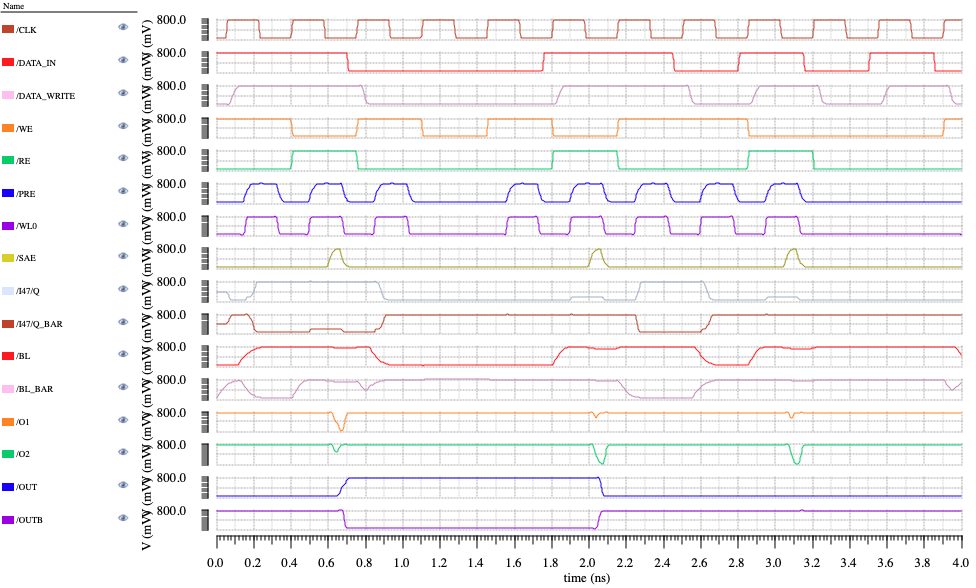
\includegraphics[clip,width=0.9\columnwidth]{Problem4-MaxFreq.png}
\caption{Read and Write Operation ($F_{CLK} = 2.86GHz$)}
\label{fig:max_freq}
\end{figure}

\clearpage
\begin{center}
\section{SRAM Problem 5: 16x4 Cell Array}
\end{center}

\subsection{Full Schematic}
\begin{figure}[h!]
\centering
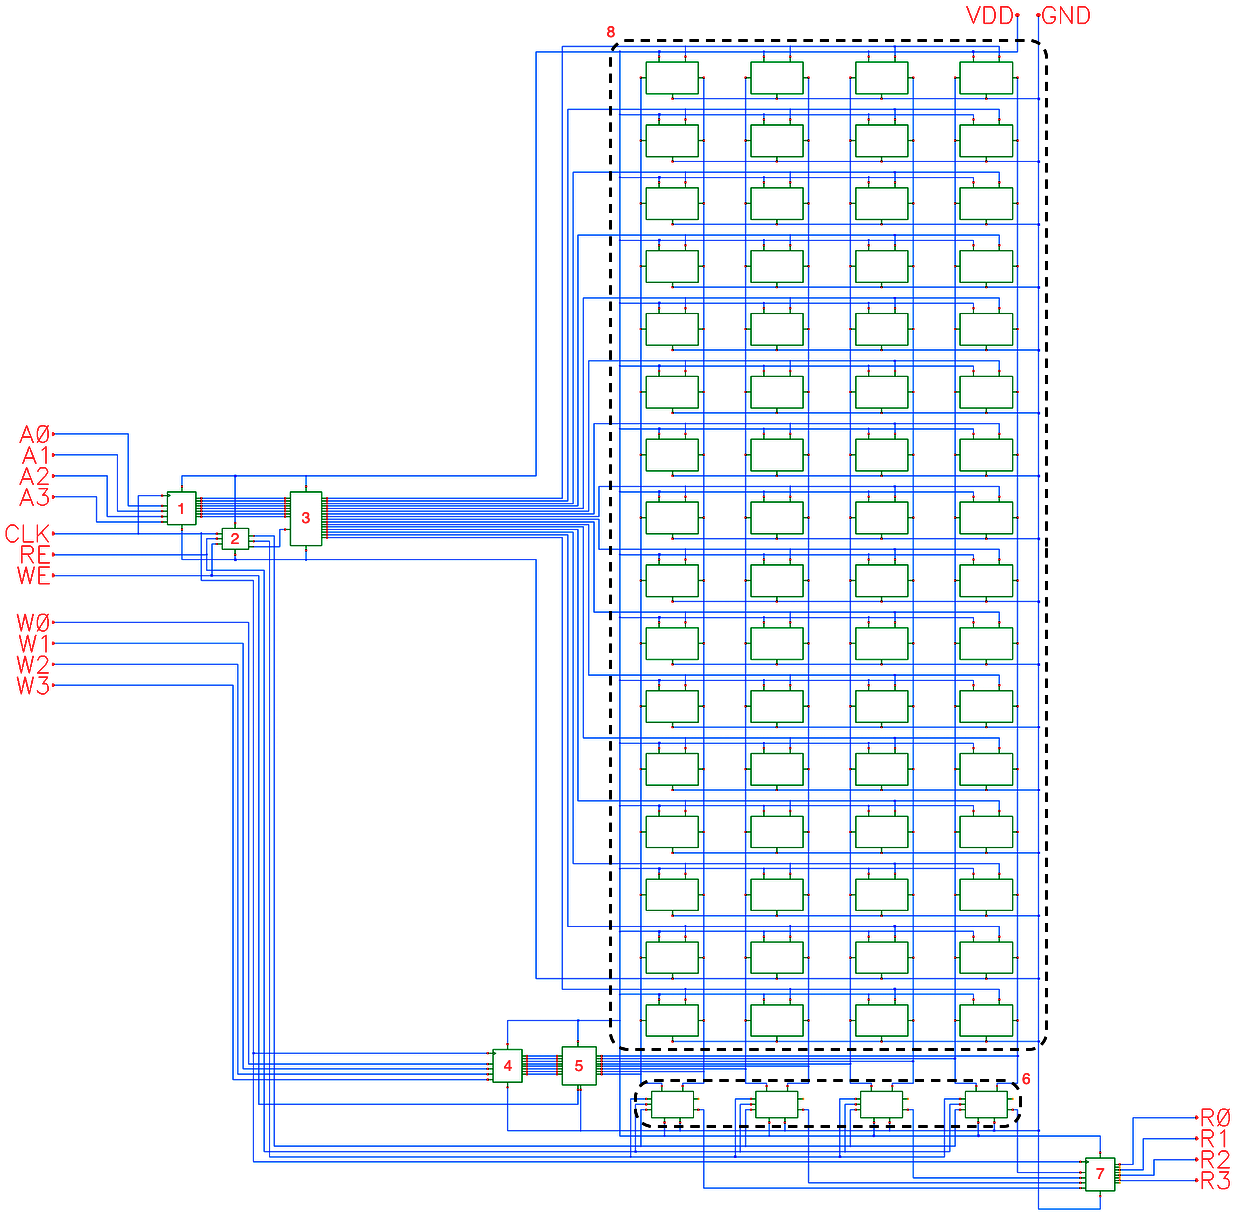
\includegraphics[clip,width=0.9\columnwidth]{Full_Schematic.png}
\caption{16x4 SRAM Cell Array with Full Peripheral}
\label{fig:Full_Schematic}
\end{figure}

\begin{table}[h!]
\centering
\begin{tabular}{ |c|l| }
  \hline
  \textbf{Item No.} & \textbf{Description} \\ 
  \hline
  1 & Address Register \\  
  \hline
  2 & Control Signal Generator \\
  \hline
  3 & Word Line Row Decoder \\
  \hline
  4 & Data Register (Write Operation) \\
  \hline
  5 & Write Circuit \\  
  \hline
  6 & Read Circuit \\
  \hline
  7 & Data Register (Read Operation) \\
  \hline
  8 & $16\times4$ SRAM Cell Array \\
  \hline
\end{tabular}
\caption{Full Schematic Devices}
\label{table:Full_Decives}
\end{table}

[A0 A1 A2 A3] is a 4-bit address input used to choose which word line to write to. [W0 W1 W2 W3] is a 4-bit data input the user may write to the SRAM cell during a write cycle. [R0 R1 R2 R3] is a 4-bit output that results from reading the SRAM cell. The CLK, RE, and WE signals are user-provided signals for clock, read enable, and write enable, respectively.

\subsection{Top Level Block Diagram}
\begin{figure}[h!]
    \centering
    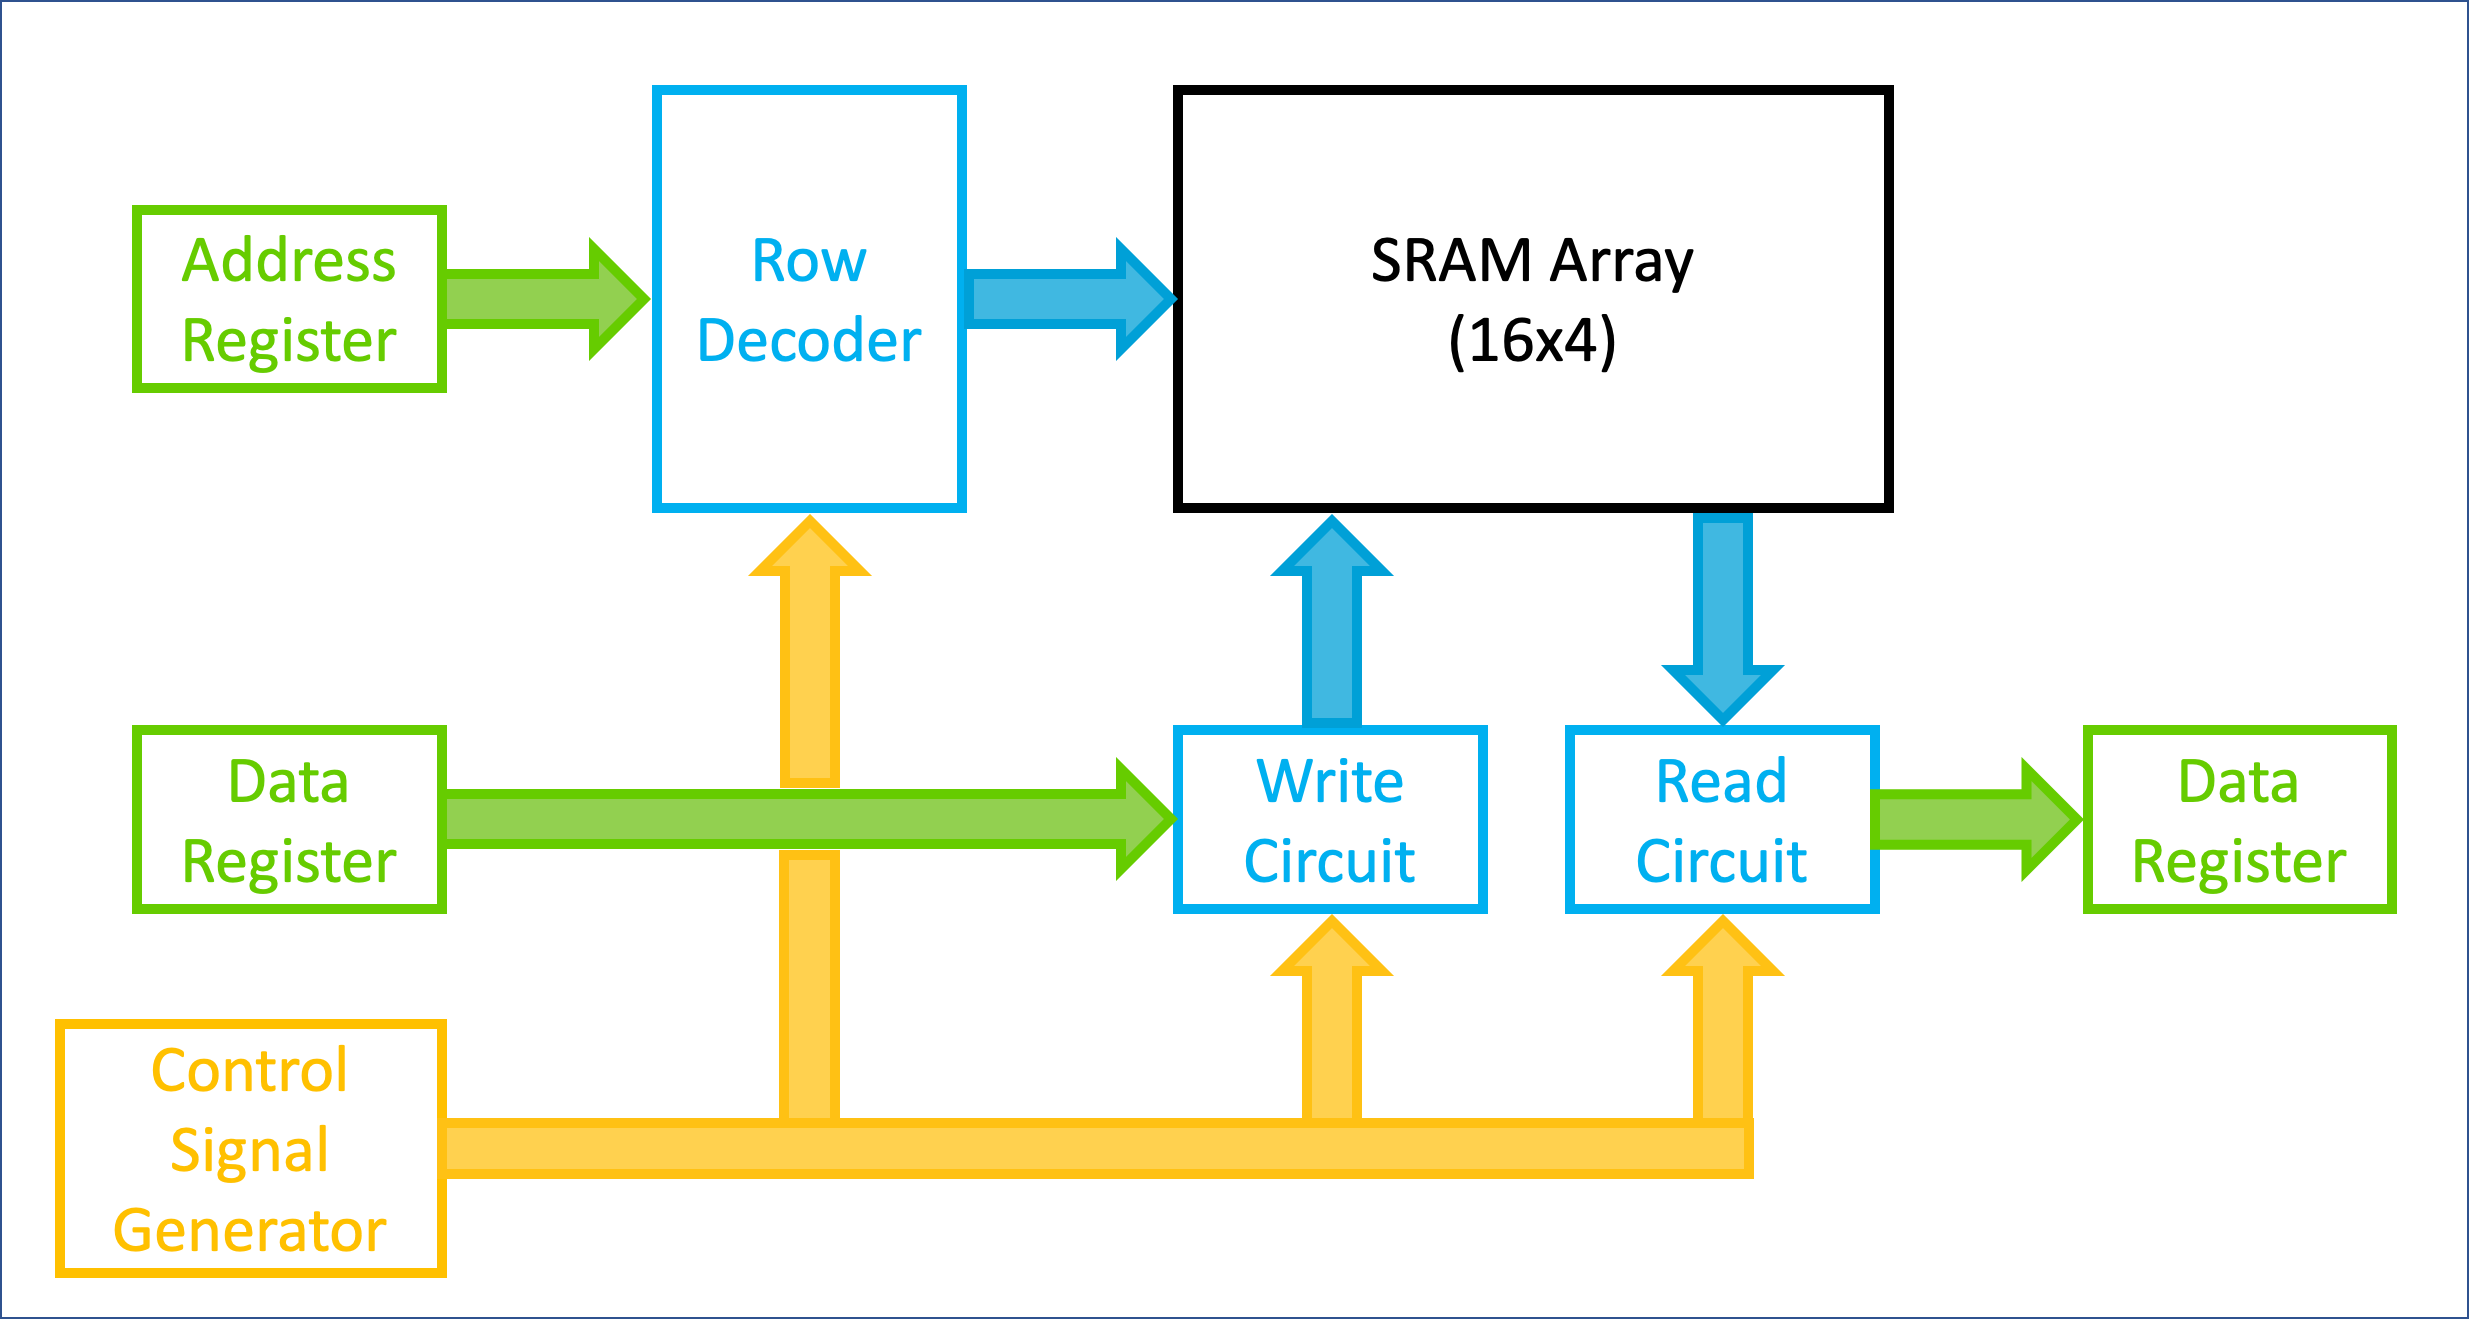
\includegraphics[clip,width=\columnwidth]{top_level_block.png}
    \caption{Top Level Block Diagram}
    \label{fig:top_level_block}
\end{figure}

\clearpage
\begin{center}
\section{Peripheral Optimizations}
\end{center}

\subsection{Row Decoder}

\subsubsection{Previous Design}

This section briefly discusses the previous design of the decoder. A NAND-NOR-INV Predecoder design was used for realizing the decoder. A critical path of WL0 is shown in Figure~\ref{fig:CriticalPath} for reference. 

\begin{figure}[h!]
\centering
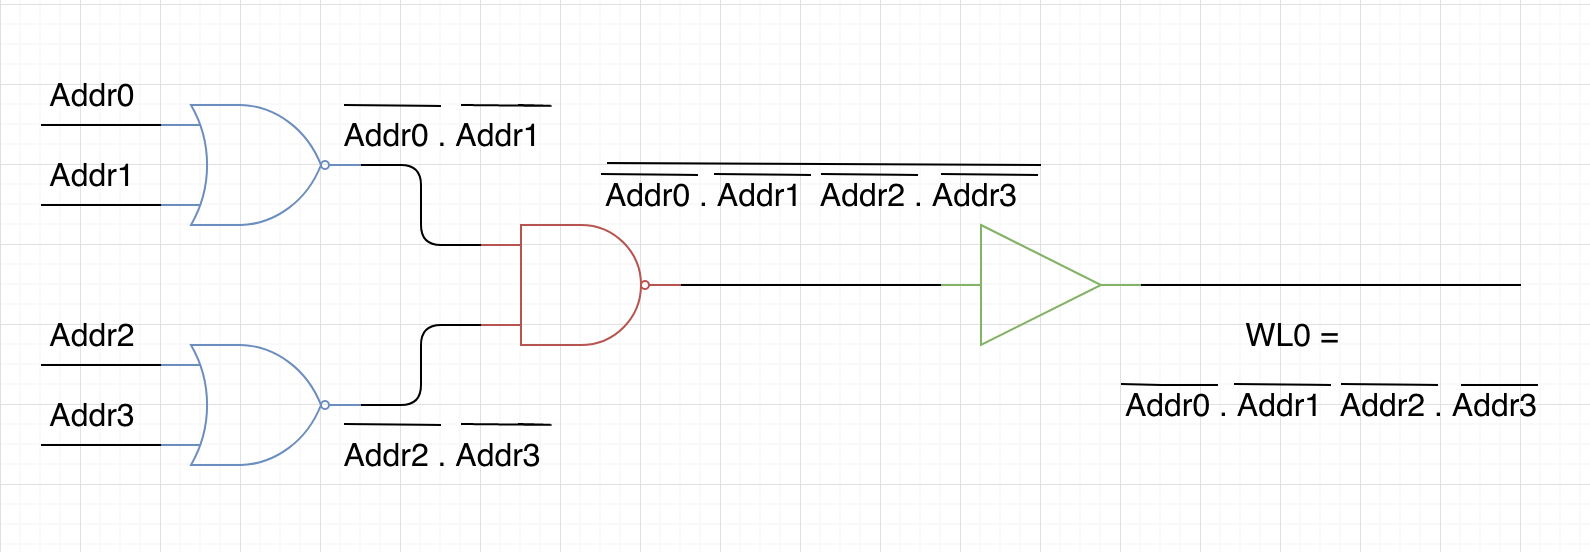
\includegraphics[scale=0.6]{CriticalPath.png}
\caption{Critical Path of WL0}
\label{fig:CriticalPath}
\end{figure}

For the synchronization with PRE signal, a different kind of dynamic inverter ( refered to as "Reverse Dynamic Inverter" from now on) was used instead of the regular Static CMOS inverter. Refer to Figure~\ref{fig:RevDynamic} for the same. This inverter takes PRE\_inv ( inverted PRE signal ) and the WL signal as the input, and outputs WL which is synced with PRE signal. In case where PRE\_inv is 1, i.e. when PRE = 0, the output defaults to 0. 

\begin{figure}[h!]
\centering
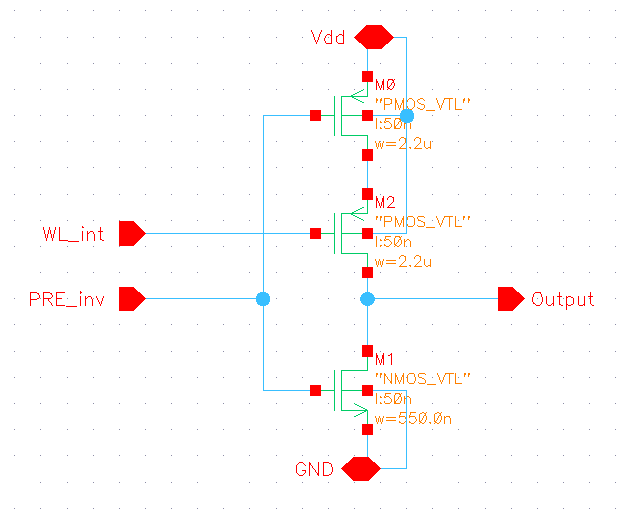
\includegraphics[scale=0.6]{RevDynamic.png}
\caption{Reverse Dynamic Inverter (non-optimized) }
\label{fig:RevDynamic}
\end{figure}

The benefit of using this circuit was synchronization of WL and PRE at low area cost and default WL = 0 condition. However when pulling up, it requires large PMOS transistors (Refer to sizing in Figure~\ref{fig:RevDynamic} ) . It has certain undesirable effects which are discussed and solved in the following section. 


\subsubsection{Improvements in Previous Design}

The drawbacks of using large pull up transistors in Reverse Dynamic Inverter are: 

\begin{enumerate}
  \item The decoder was causing higher power consumption.
  \item Synchronization was generating voltage undershoot spikes
  \item Large gate capacitance of pull up PMOS was causing unnecessary loading on PRE generator circuitry.
\end{enumerate} \\
To mitigate these problems, transistor sizing were reduced ( based on parametric analysis with trade off between delay and size ). But in addition to that, one more design modification was also introduced. This new design exploits the fact that at any one time, maximum 1 WL line needs to be pulled up. Not more than that. In the previous design, large Pull Up Transistors were attached to all WL lines, but in the new design we reduce the size as well as the transistor count by introducing a common pull up network. \\

\begin{figure}[h!]
\centering
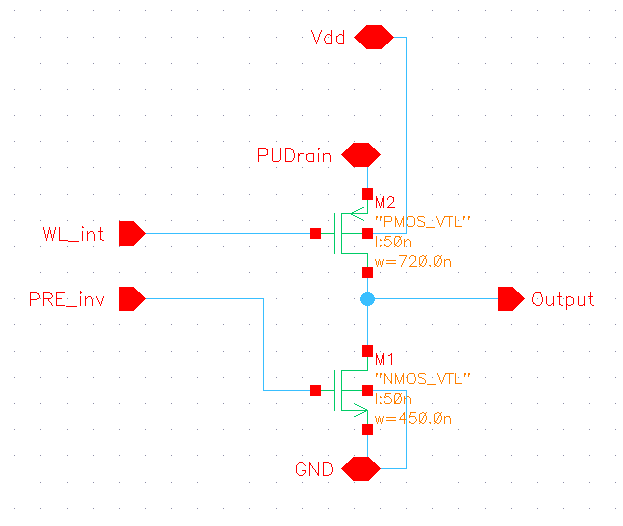
\includegraphics[scale=0.6]{RevDynamicNew.png}
\caption{Reverse Dynamic Inverter (Shared Pull-Up) }
\label{fig:RevDynamicNew}
\end{figure}

As seen in the figure above, one large pull up transistor is removed. And instead of it, the source of PMOS M2 is connected to the Drain of the common pull up network. (Refer to Figure~\ref{fig:RevDynamicCircuit}).  This design update combines all the pull ups into one single pull up node. \\ \\  Figure~\ref{fig:RevDynamicCircuit} shows common pull up implementation for 1 WL line. Here, PUDrain signal is common to all WL producing inverters. WL0\_int is the non-synchronized WL output from the previous logic. Which gets synchronized with PRE signal at the output of this Inverter. This implementation is repeated for all WL lines, keeping the PUDrain node common. \\ \\
The benefits of using common pull up is,
\begin{enumerate}
  \item Reduction of 13 transistors ( 3 common pull up PMOS, instead of 16 individual WL PMOS )  
  \item Reduced transistor sizing ( from 2.2$\mu$ PMOS \& 550n NMOS to 720n PMOS \& 450n NMOS)
  \item Reduced power consumption (from 41 $\mu$W to 31.8 $\mu$W) 
\end{enumerate}


\begin{figure}[h!]
\centering
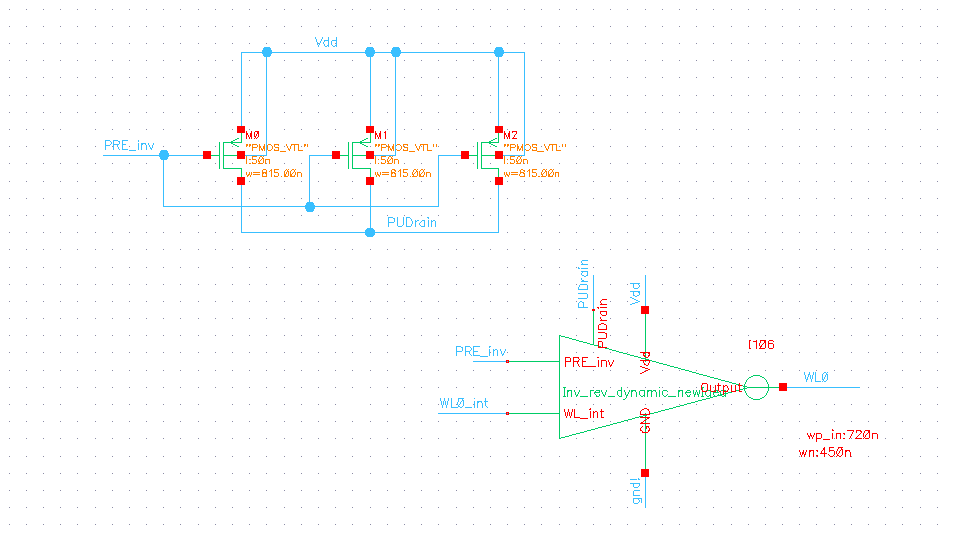
\includegraphics[scale=0.6]{RevDynamicCircuit.png}
\caption{ Common Pull Up Inverter Implementation }
\label{fig:RevDynamicCircuit}
\end{figure}


\subsubsection{Power Consumption}

Part of the reason for the implementing above mentioned optimization, was to reduce the power consumption as large transistors consume more power. The decoder outputs were simulated for the full truth table ( i.e. WL0 to WL15 ) in ascending as well as descending order. In both the cases, simulation ran for 6.4 ns ( 400 ps clock period $\times$ 16 different inputs = 6.4 ns). \\
Switching Factor (number of inputs changing at a time) varies from minimum 1 (output switching from WL0 to WL1) to maximum 4 (output switching from WL7 to WL8). \\ 
The final result is as below,
\begin{itemize}
  \item Power Consumption ( Ascending Truth Table ) : $31.8 \; \mu W$
  \item Power Consumption ( Descending Truth Table ) : $31.8 \; \mu W$
\end{itemize} \\
Figure~\ref{fig:DecoderTruthTable} shows the Decoder Output simulation for which average power consumption was calculated. Note that here, WL is not synchronized with PRE signal. For the purpose of power consumption calculation, only correct functionality of WL is checked for all possible input combinations. 

\begin{figure}[h!]
\centering
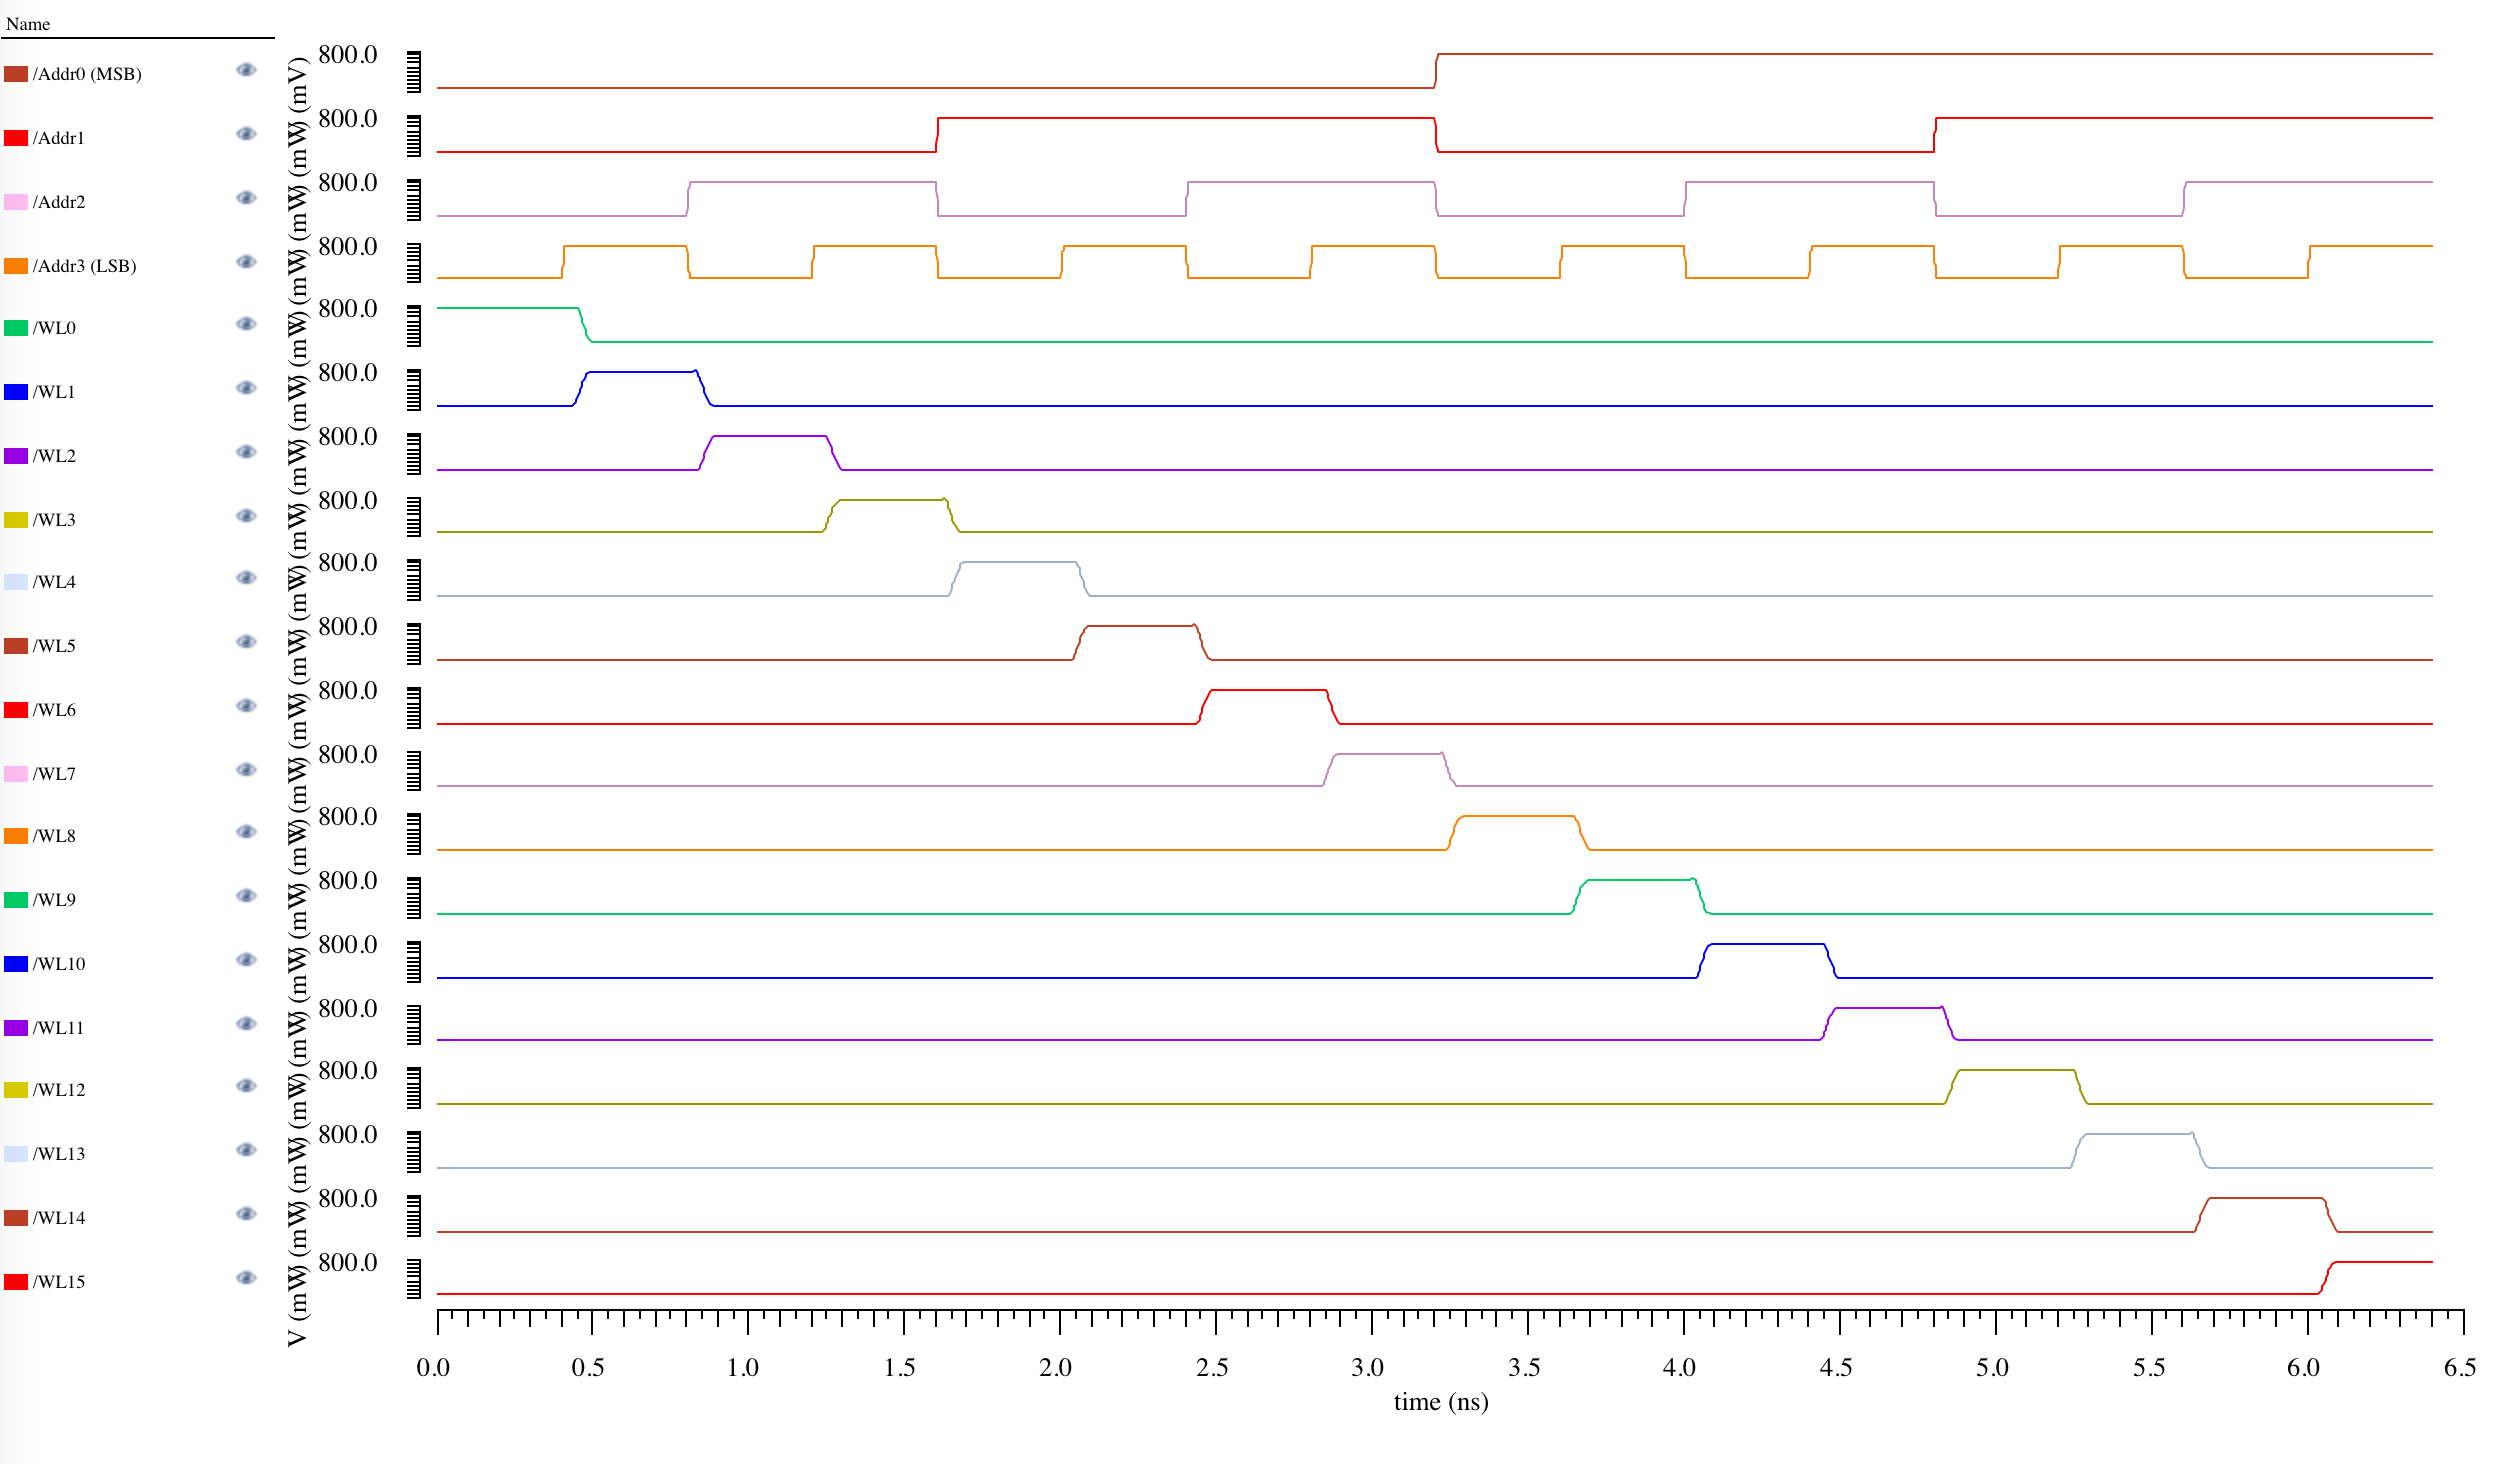
\includegraphics[scale=0.4]{DecoderTruthTableAscending.png}
\caption{Ascending Truth Table of Decoder for Power Calculation}
\label{fig:DecoderTruthTable}
\end{figure}


\subsection{Register}
\subsubsection{Schematic and size}
In this report, we improved our register in two perspectives. One is to make the C-Q delay of low-to-high and high-to-low balanced. Another one is to size it down to get a lower power consumption.\\
Optimization of the flip-flop involved trying to balance the C-Q delay for high-to-low and low-to-high transitions. The results are shown in Figure~\ref{fig:CQDelay}. In the previous flip-flop design, the low-to-high delay was shorter than the high-to-low delay. To fix this issue, we sized up the pull-down network. In addition, we made the farthest NMOS a little larger for a stronger pull-down, as seen in Figure~\ref{fig:NAND2}.\\
For power consumption, we got $64.33 \mu W$ in our previous report. In this report, since the smaller transistors, we had a better result. \\
The new specifications for the register are as follows:
\begin{itemize}
  \item C-Q Delay: 28.5 ps
  \item Setup Time: 35 ps
  \item Hold Time: 0 ps
  \item Power Consumption - Four Bits Switching (Figure~\ref{fig:RegisterPower1}): $49.84 \mu W$
  \item Power Consumption - Average Case (Figure~\ref{fig:RegisterPower2}): $44.15 \mu W$
\end{itemize}

Figure~\ref{fig:RegisterPower1} shows the simulation for how average power consumption of a register was calculated. This tested when four bits changed either from low to high or from high to low. On the other hand, since sometimes the output data might not change, so we also do this test which is shown in Figure~\ref{fig:RegisterPower2}. In Figure~\ref{fig:RegisterPower2}, A0 changed from high to low; A1 kept in high; A2 changed from low to high; A3 kept in low.

\begin{figure}[h!]
\centering
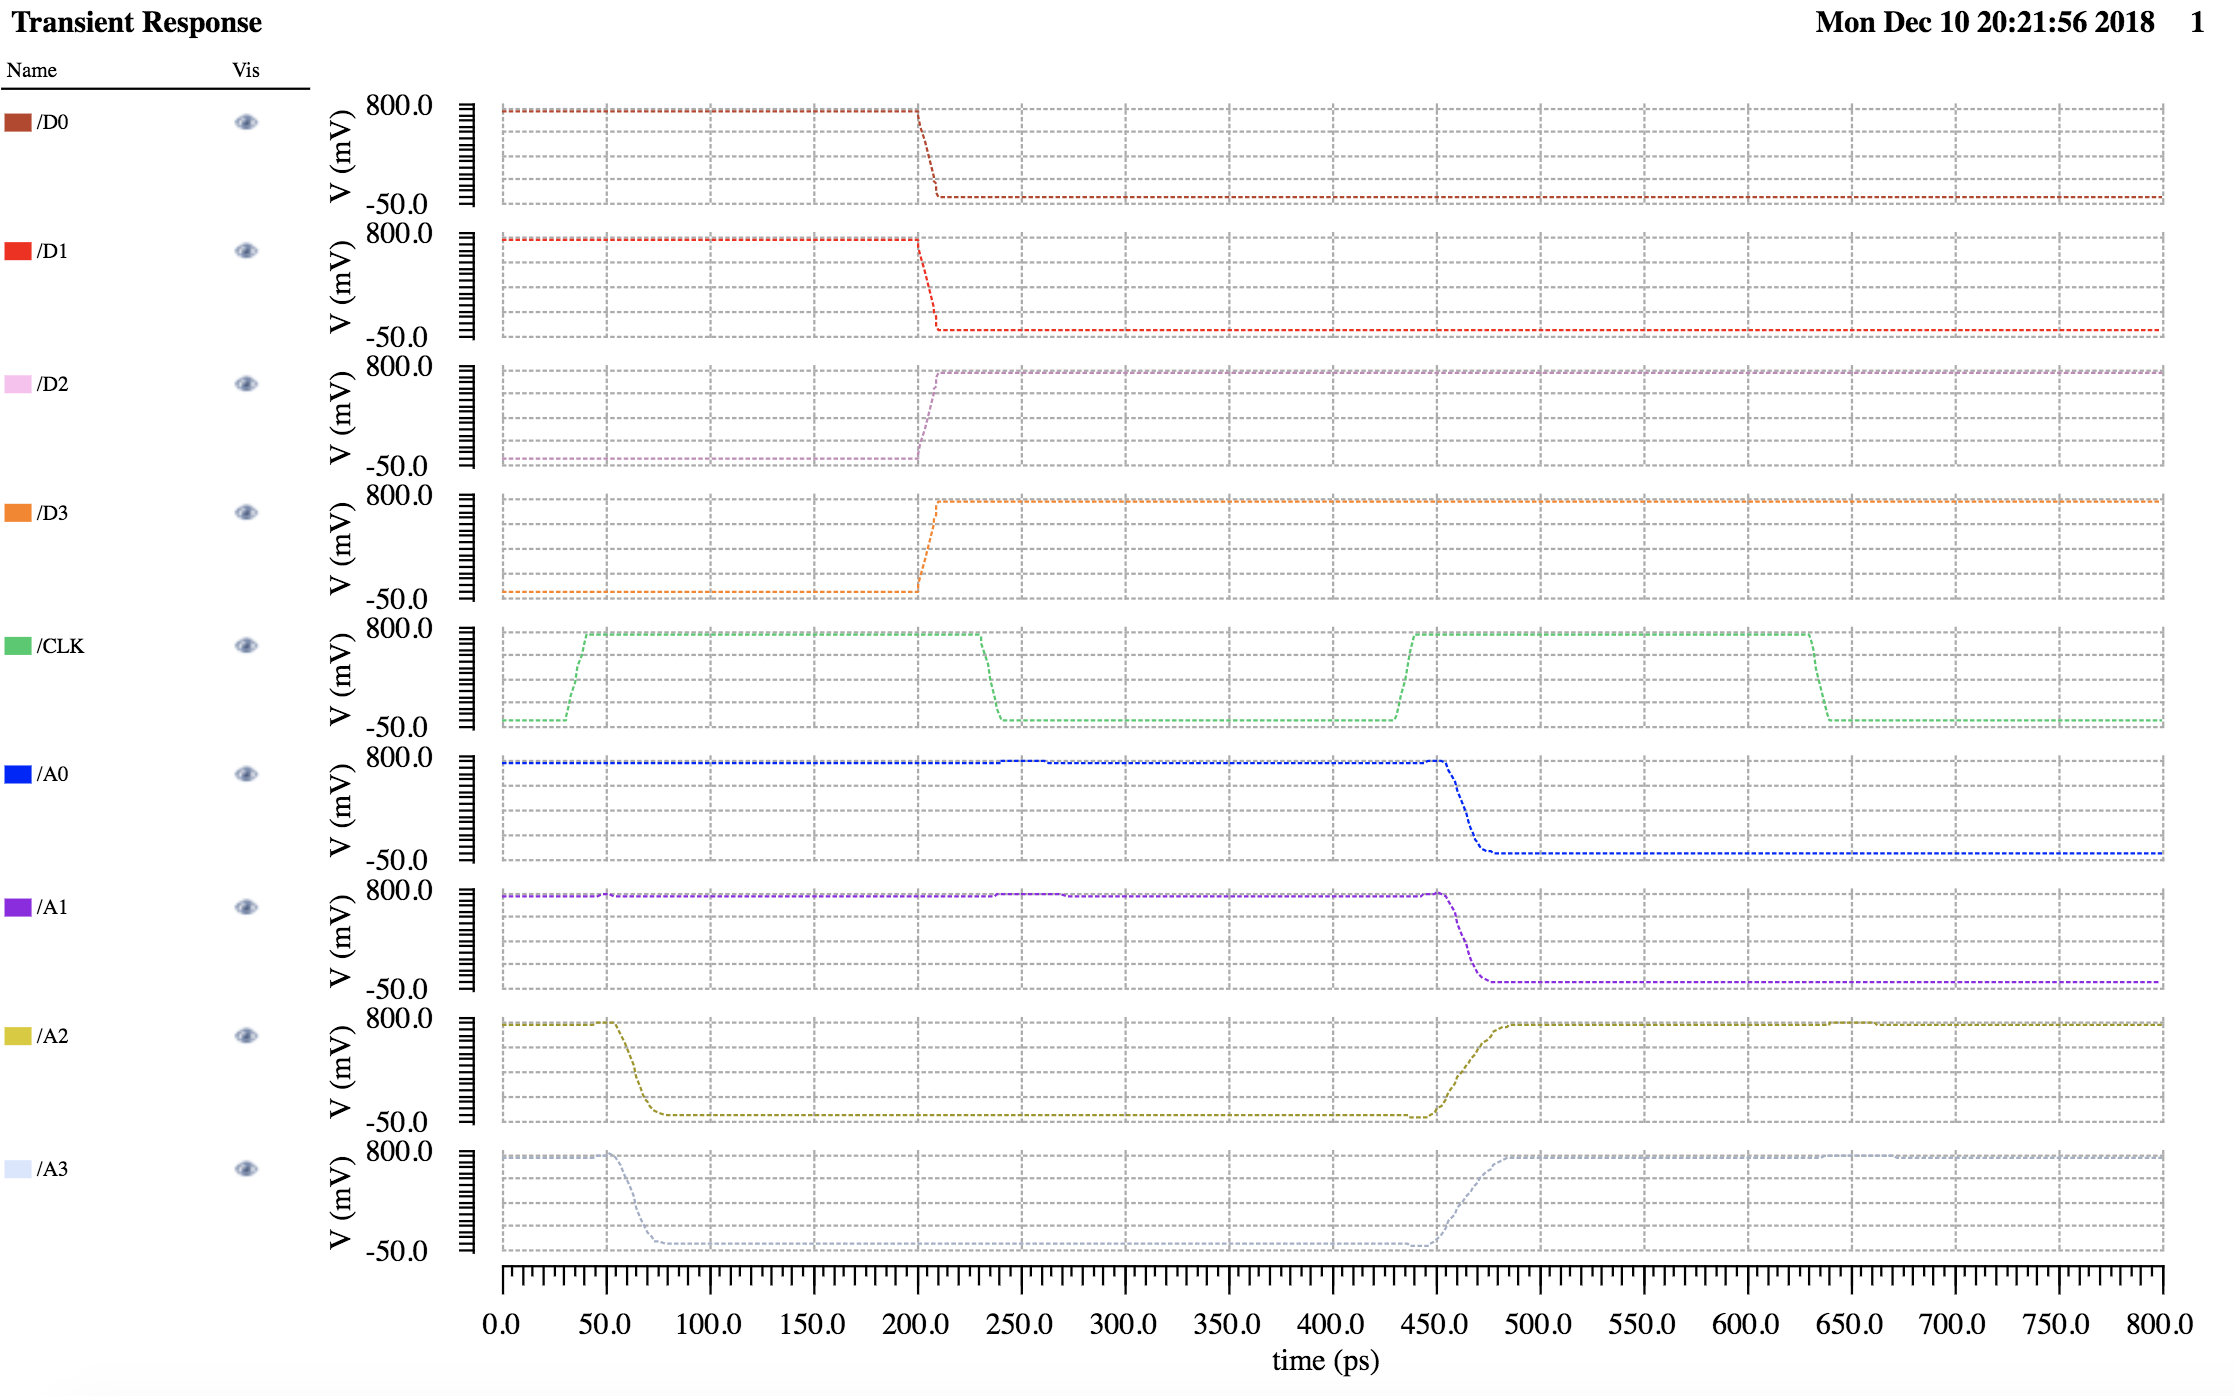
\includegraphics[clip,width=\columnwidth]{RegisterPower.png}
\caption{Register Power Calculation - Four Bits Switching}
\label{fig:RegisterPower1}
\end{figure}

\begin{figure}[h!]
\centering
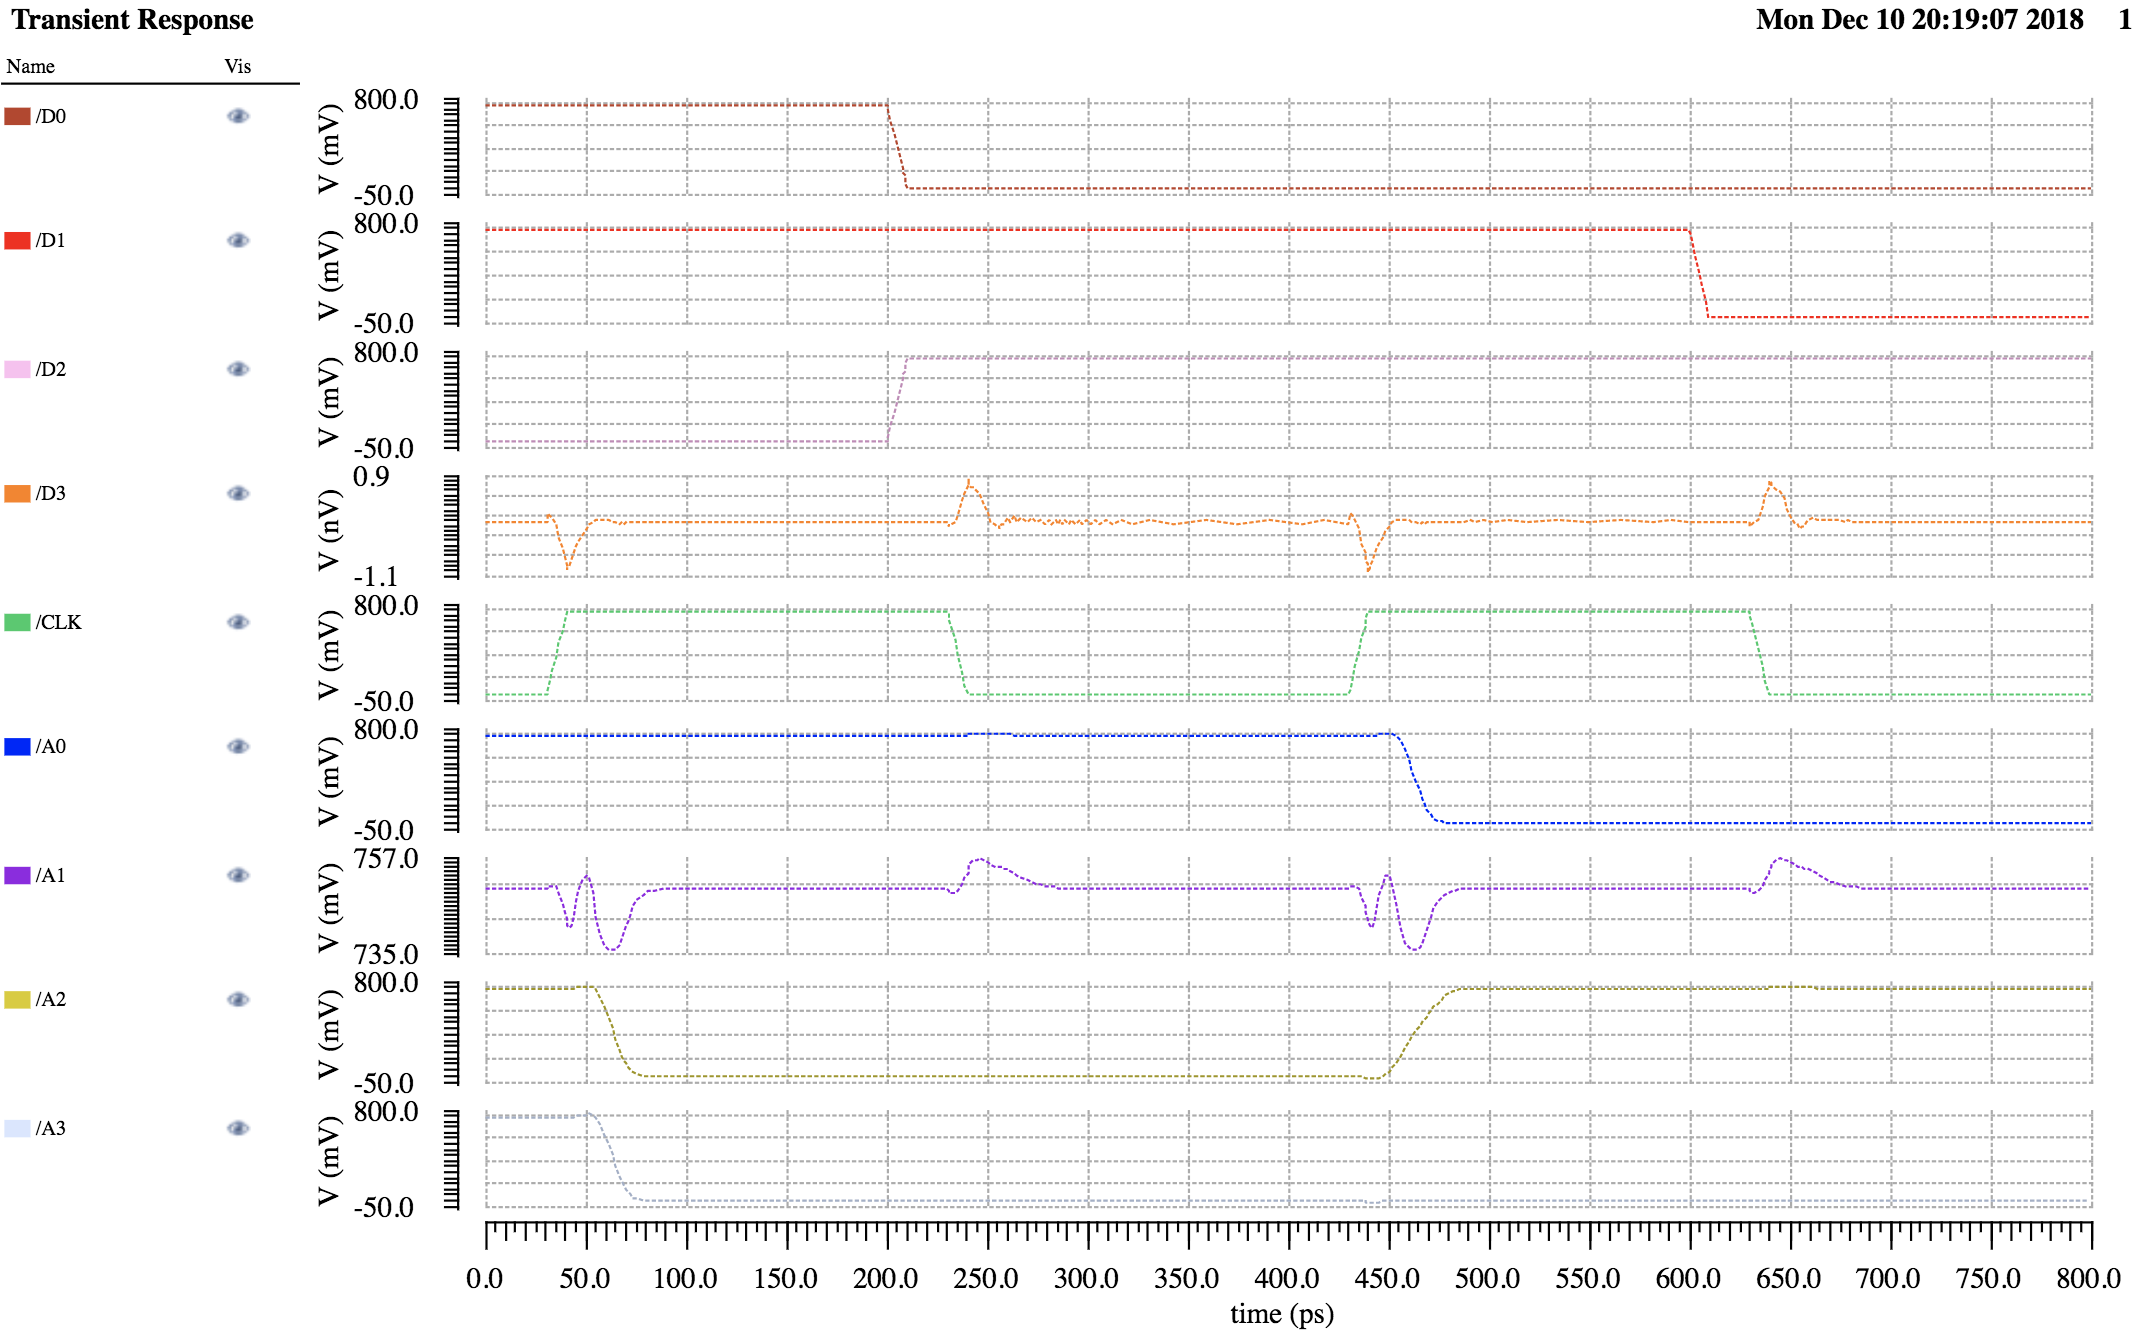
\includegraphics[clip,width=\columnwidth]{RegisterPower2.png}
\caption{Register Power Calculation - Average case}
\label{fig:RegisterPower2}
\end{figure}

\begin{figure}[h!]
\centering
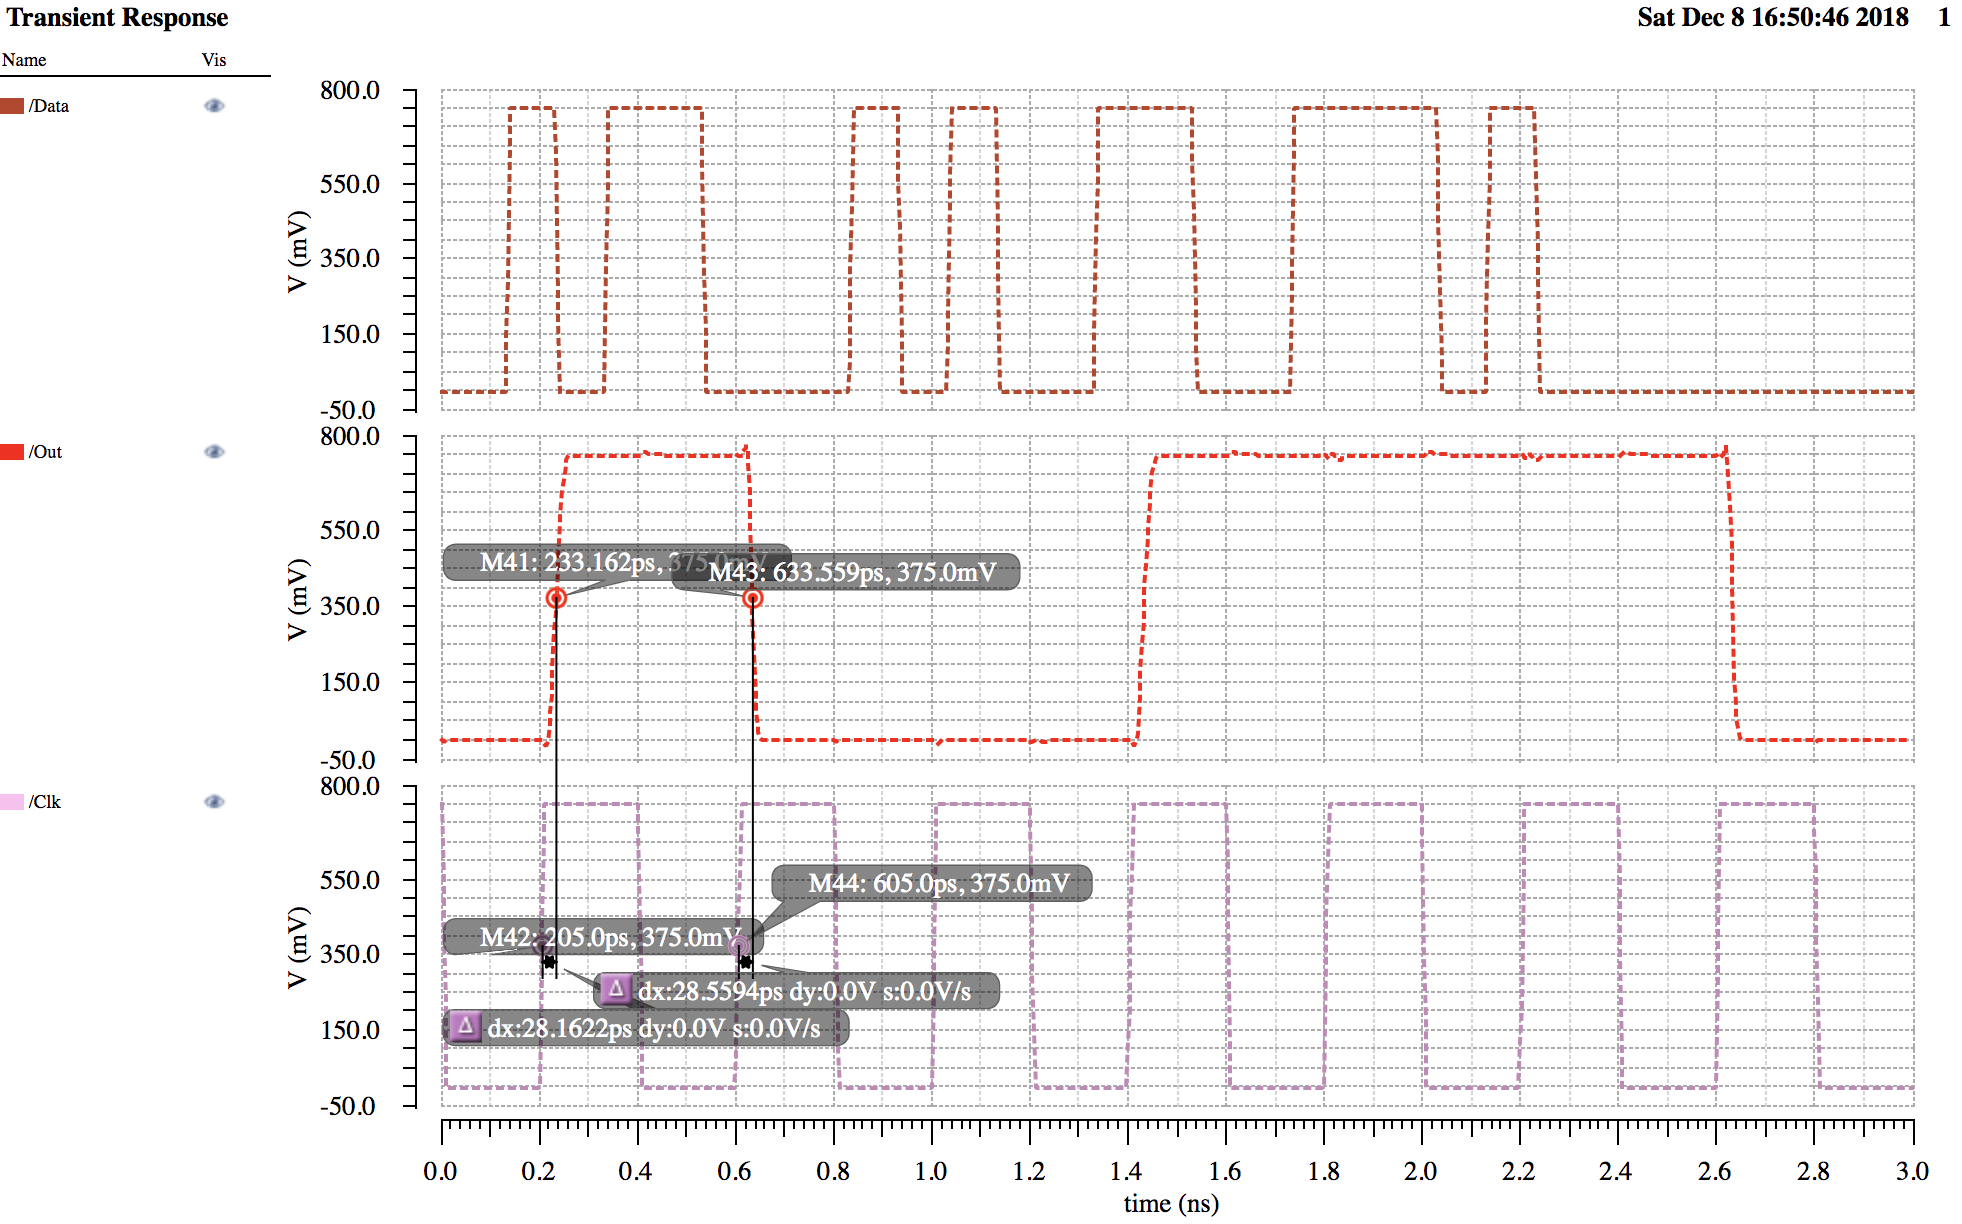
\includegraphics[clip,width=\columnwidth]{CQDelay.png}
\caption{Clk-Q delay}
\label{fig:CQDelay}
\end{figure}

\begin{figure}[h!]
\centering
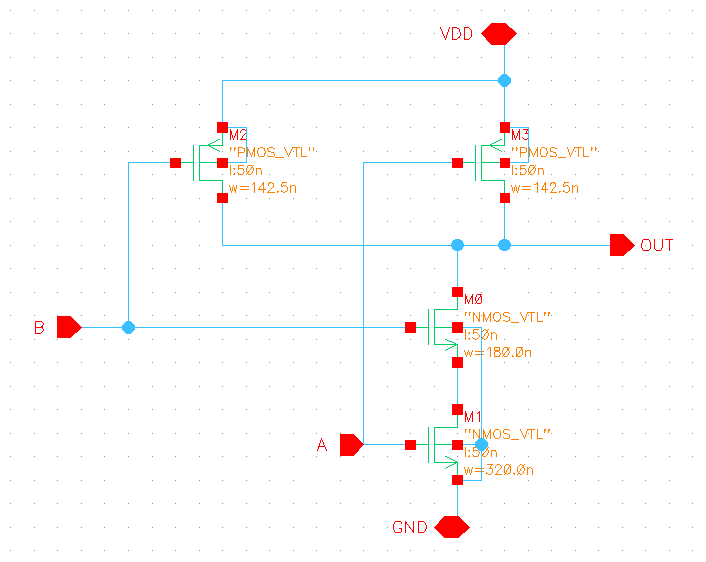
\includegraphics[clip,width=0.6\columnwidth]{NAND2.png}
\caption{Register NAND2 Gate - Schematic}
\label{fig:NAND2}
\end{figure}

\subsection{Write Circuit}

For the write circuit, we worked to optimize the sizing for both the transmission gate and the inverter. \\
To find out the relation of inverter chain and delay, we set the size of transmission gate as 800nm, and tried different inverter chain ratio. Figure~\ref{fig:inverterChainRatio} shows our testing result. \\
Based on this result, we chose \(e \times 1.7\) as the inverter chain ratio. The widths in the first stage are 245nm for NMOS ad 385nm for PMOS. The widths in the second stage are 1128nm for NMOS and 1773nm for PMOS. Compared to our previous values, we reduced the size to 63\% of the previous sizes, but still kept the delay within 100p sec.\\
Figure~\ref{fig:WEtoBL} shows the testing results of one bit write circuit connected to flip-flop.\\

\begin{figure}[h!]
\centering
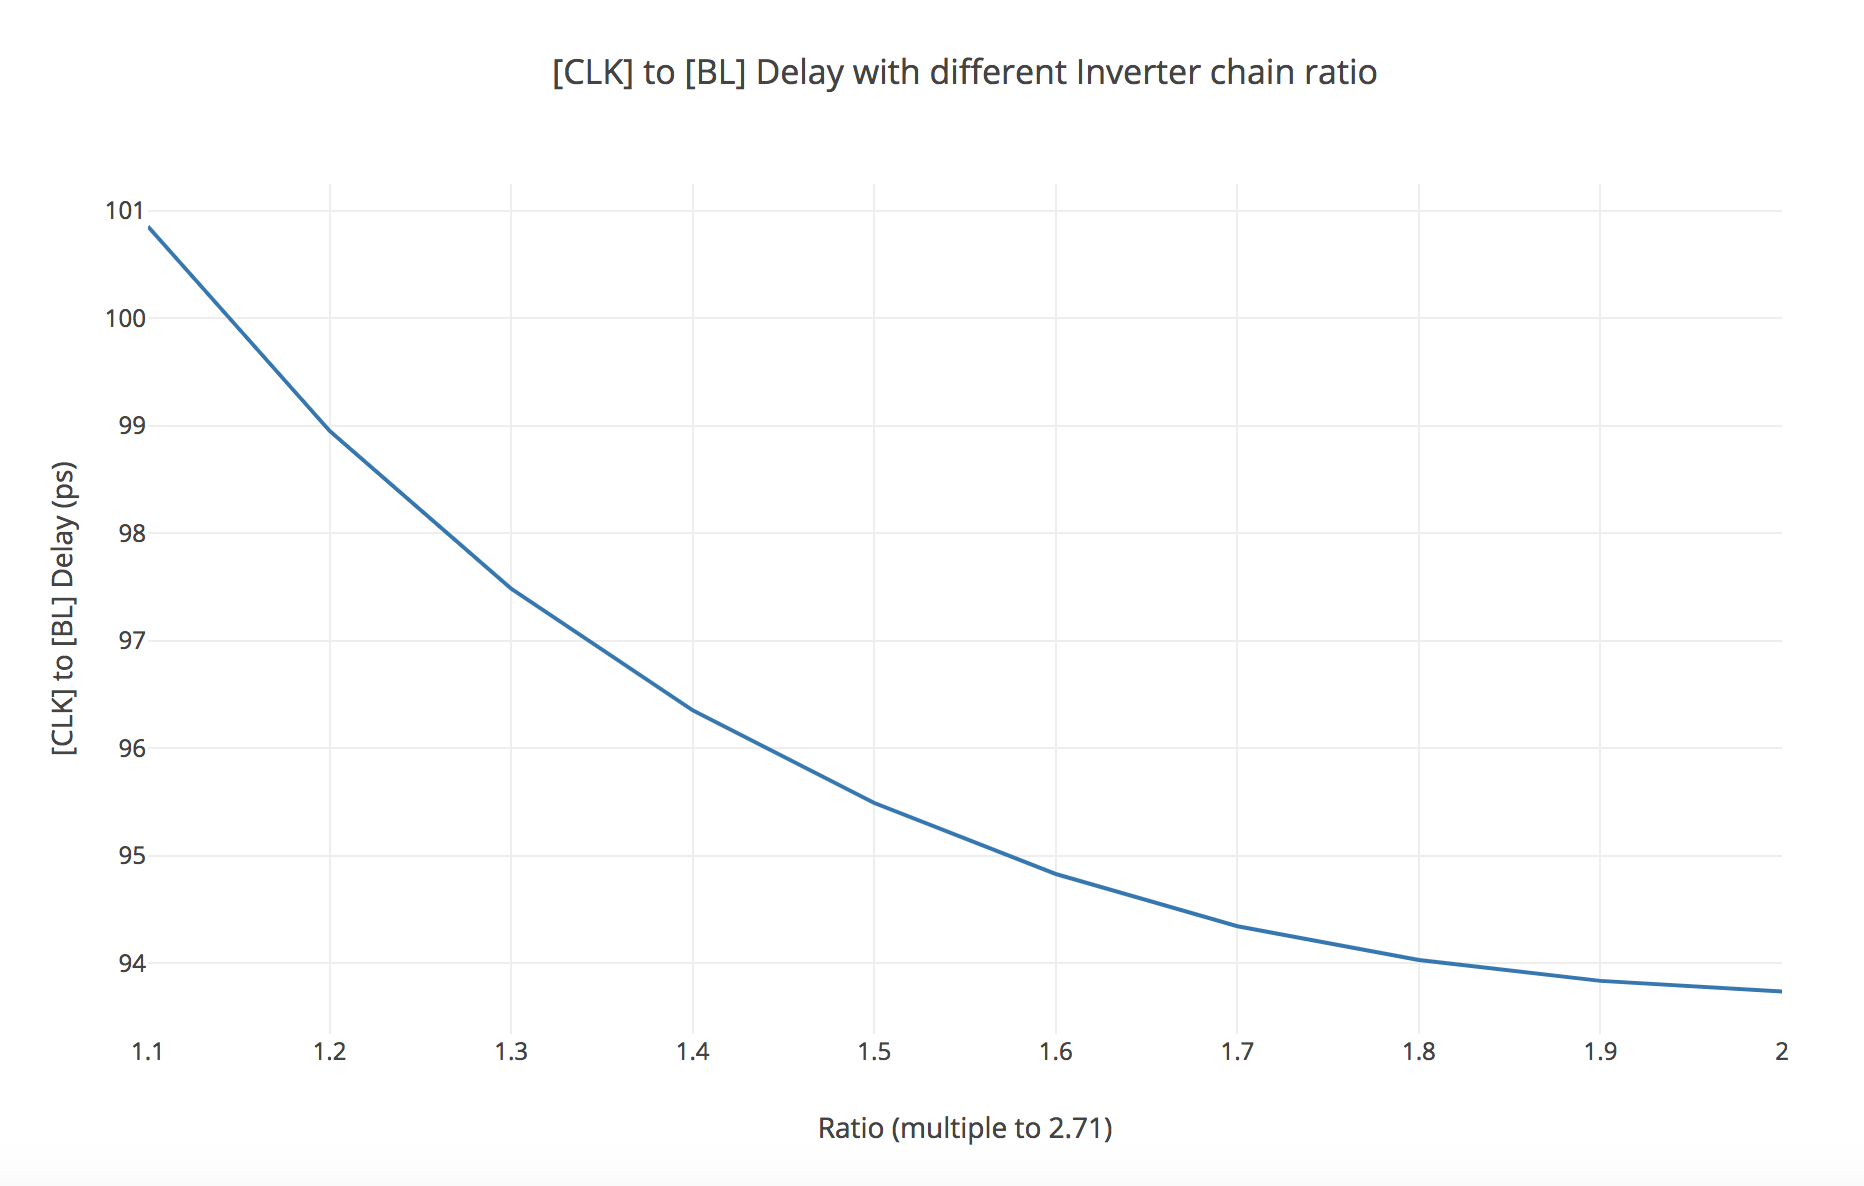
\includegraphics[clip,width=\columnwidth]{inverterChainRatio.png}
\caption{CLK to BL Delay vs. Inverter Chain Ratio}
\label{fig:inverterChainRatio}
\end{figure}

\begin{figure}[h!]
\centering
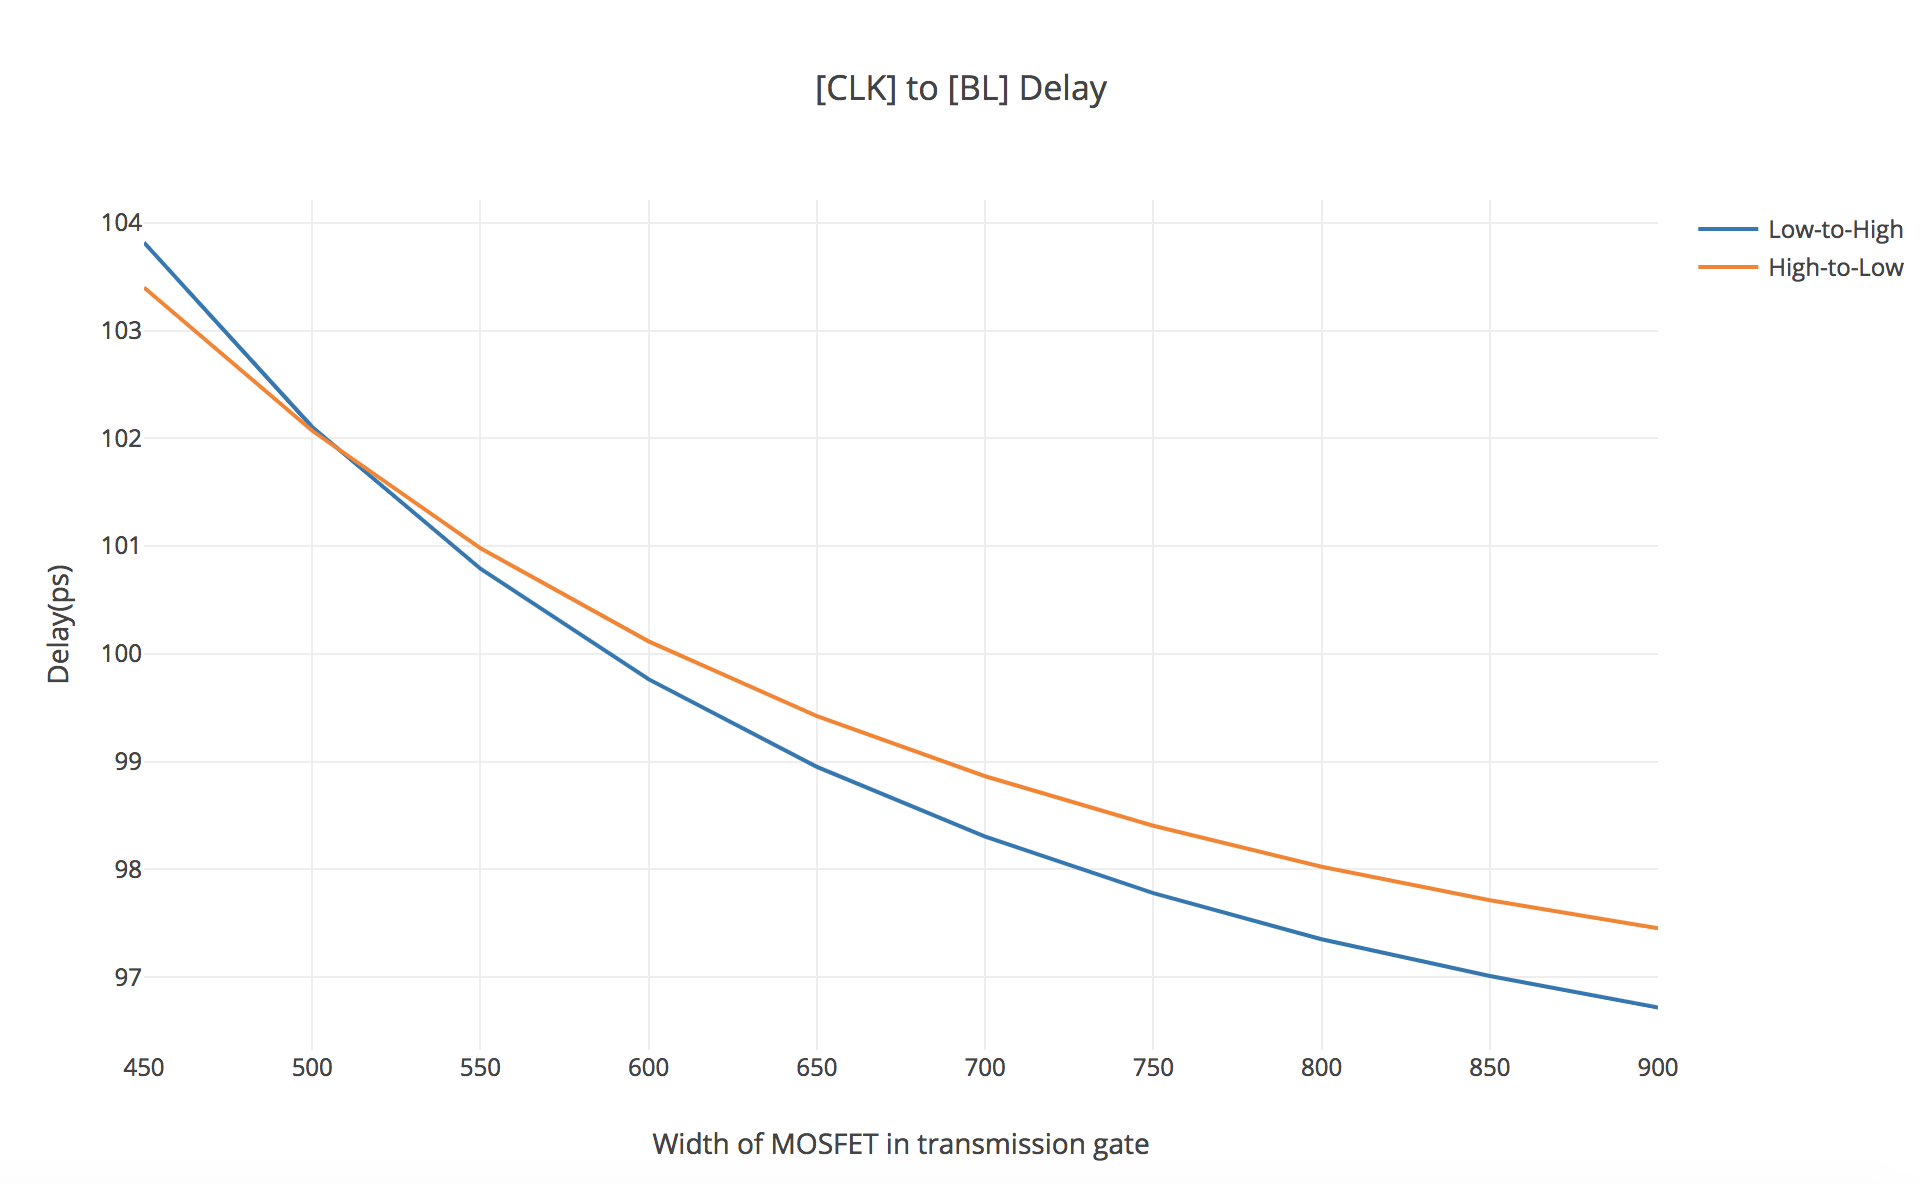
\includegraphics[clip,width=\columnwidth]{CLKtoBLDelayPlot.png}
\caption{CLK to BL Delay vs. Transmission Gate Sizing}
\label{fig:CLKtoBLPlot}
\end{figure}

\begin{figure}[h!]
\centering
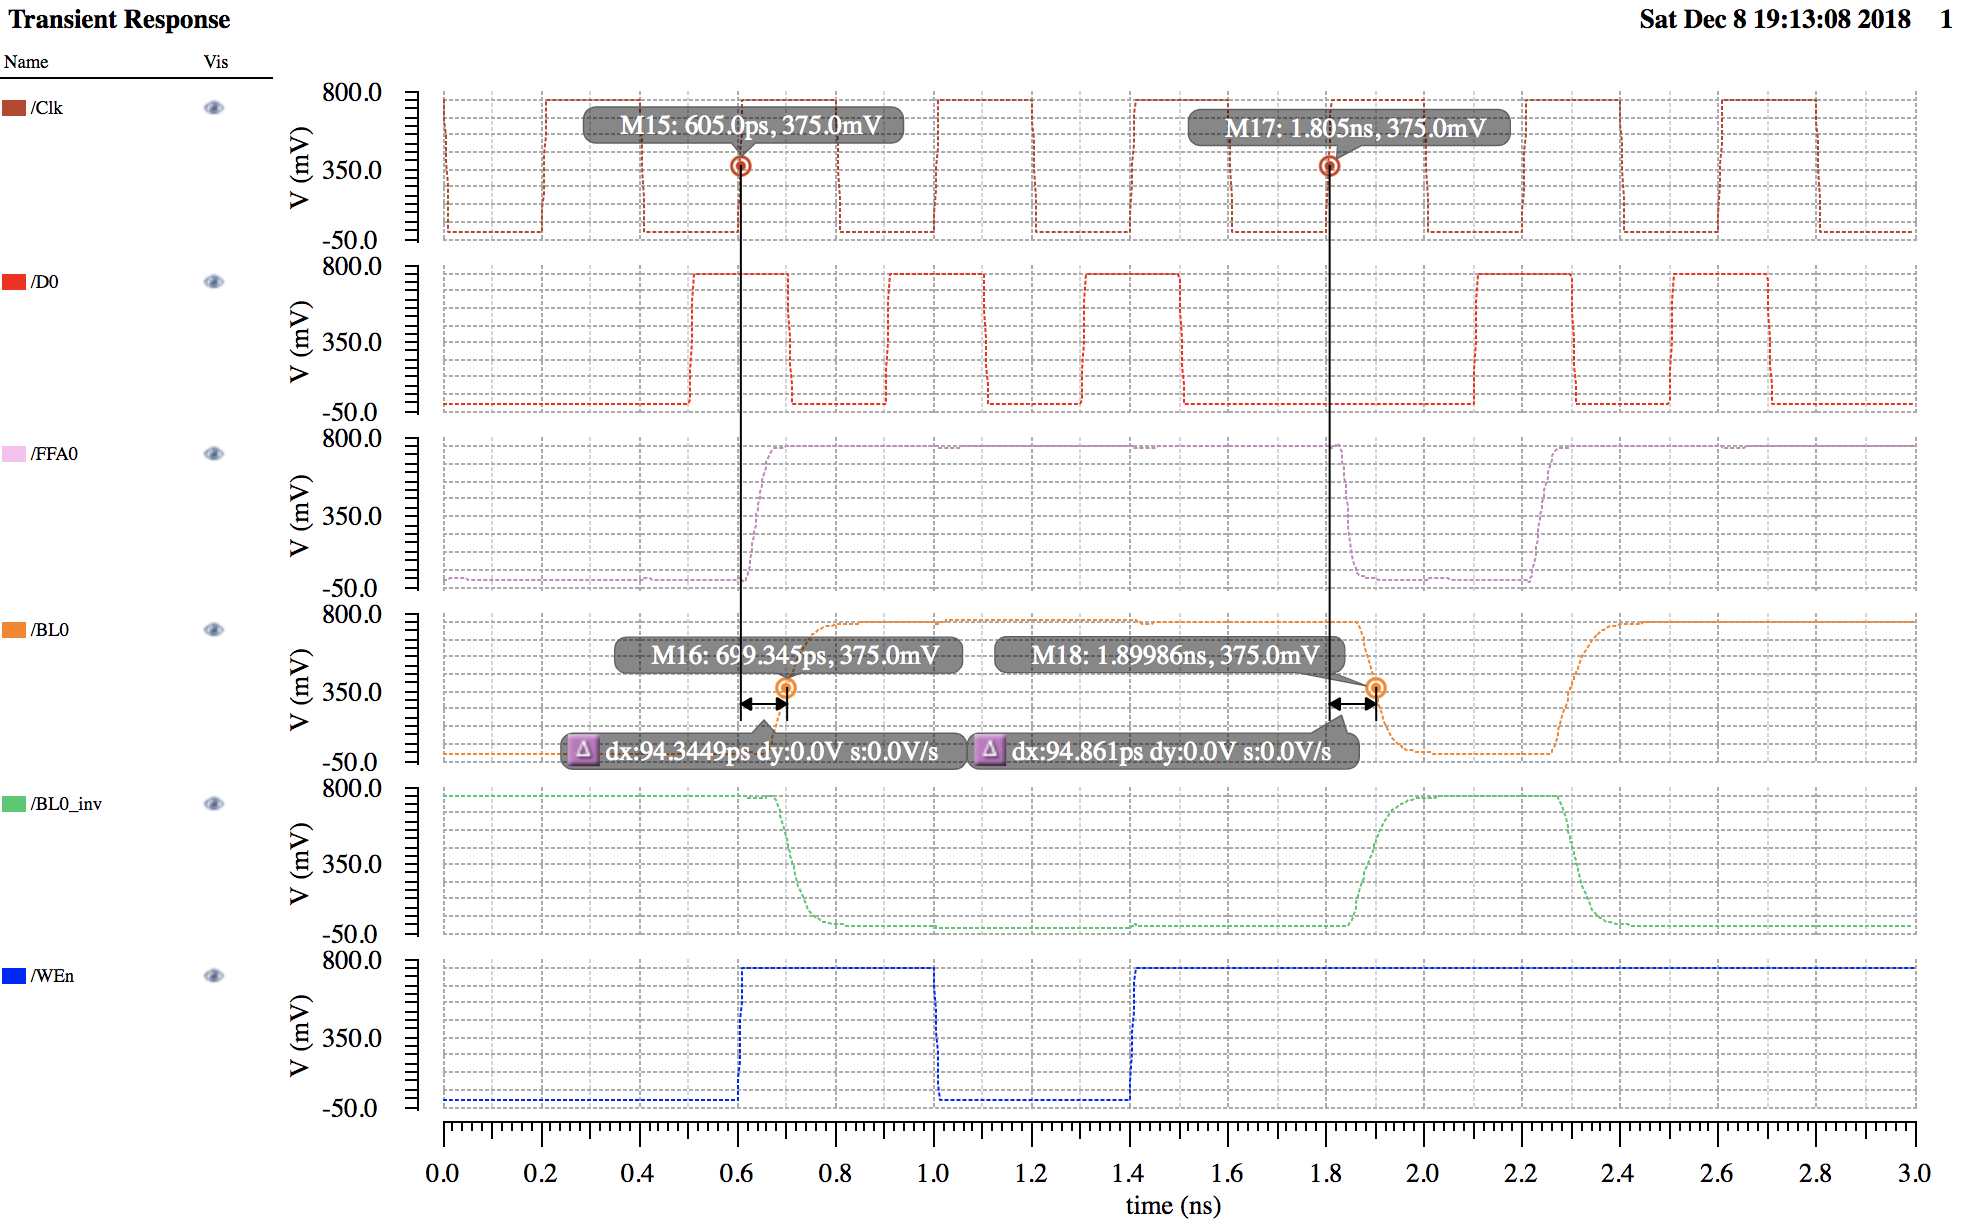
\includegraphics[clip,width=\columnwidth]{WEtoBL.png}
\caption{Single Bit Write Operation}
\label{fig:WEtoBL}
\end{figure}

\clearpage
\begin{center}
\addcontentsline{toc}{section}{APPENDIX}
\section*{APPENDIX}
\end{center}


\subsection*{Appendix A}
\subsubsection*{1. Read Noise Margin Testing}
As discussed in the section 3.2.1, two tests are needed to verify the read noise margin for every width ratio of $W_{Access}:W_{PullUp}:W_{PullDown}$ that is tested. Figure~\ref{fig:Vread_Vtrip} shows the DC analyses used to find the read voltage \& read current, and trip voltage, respectively.
\begin{figure}[htp]
    \centering
    \subfloat[{Test Circuit for $V_{read}$}]{
    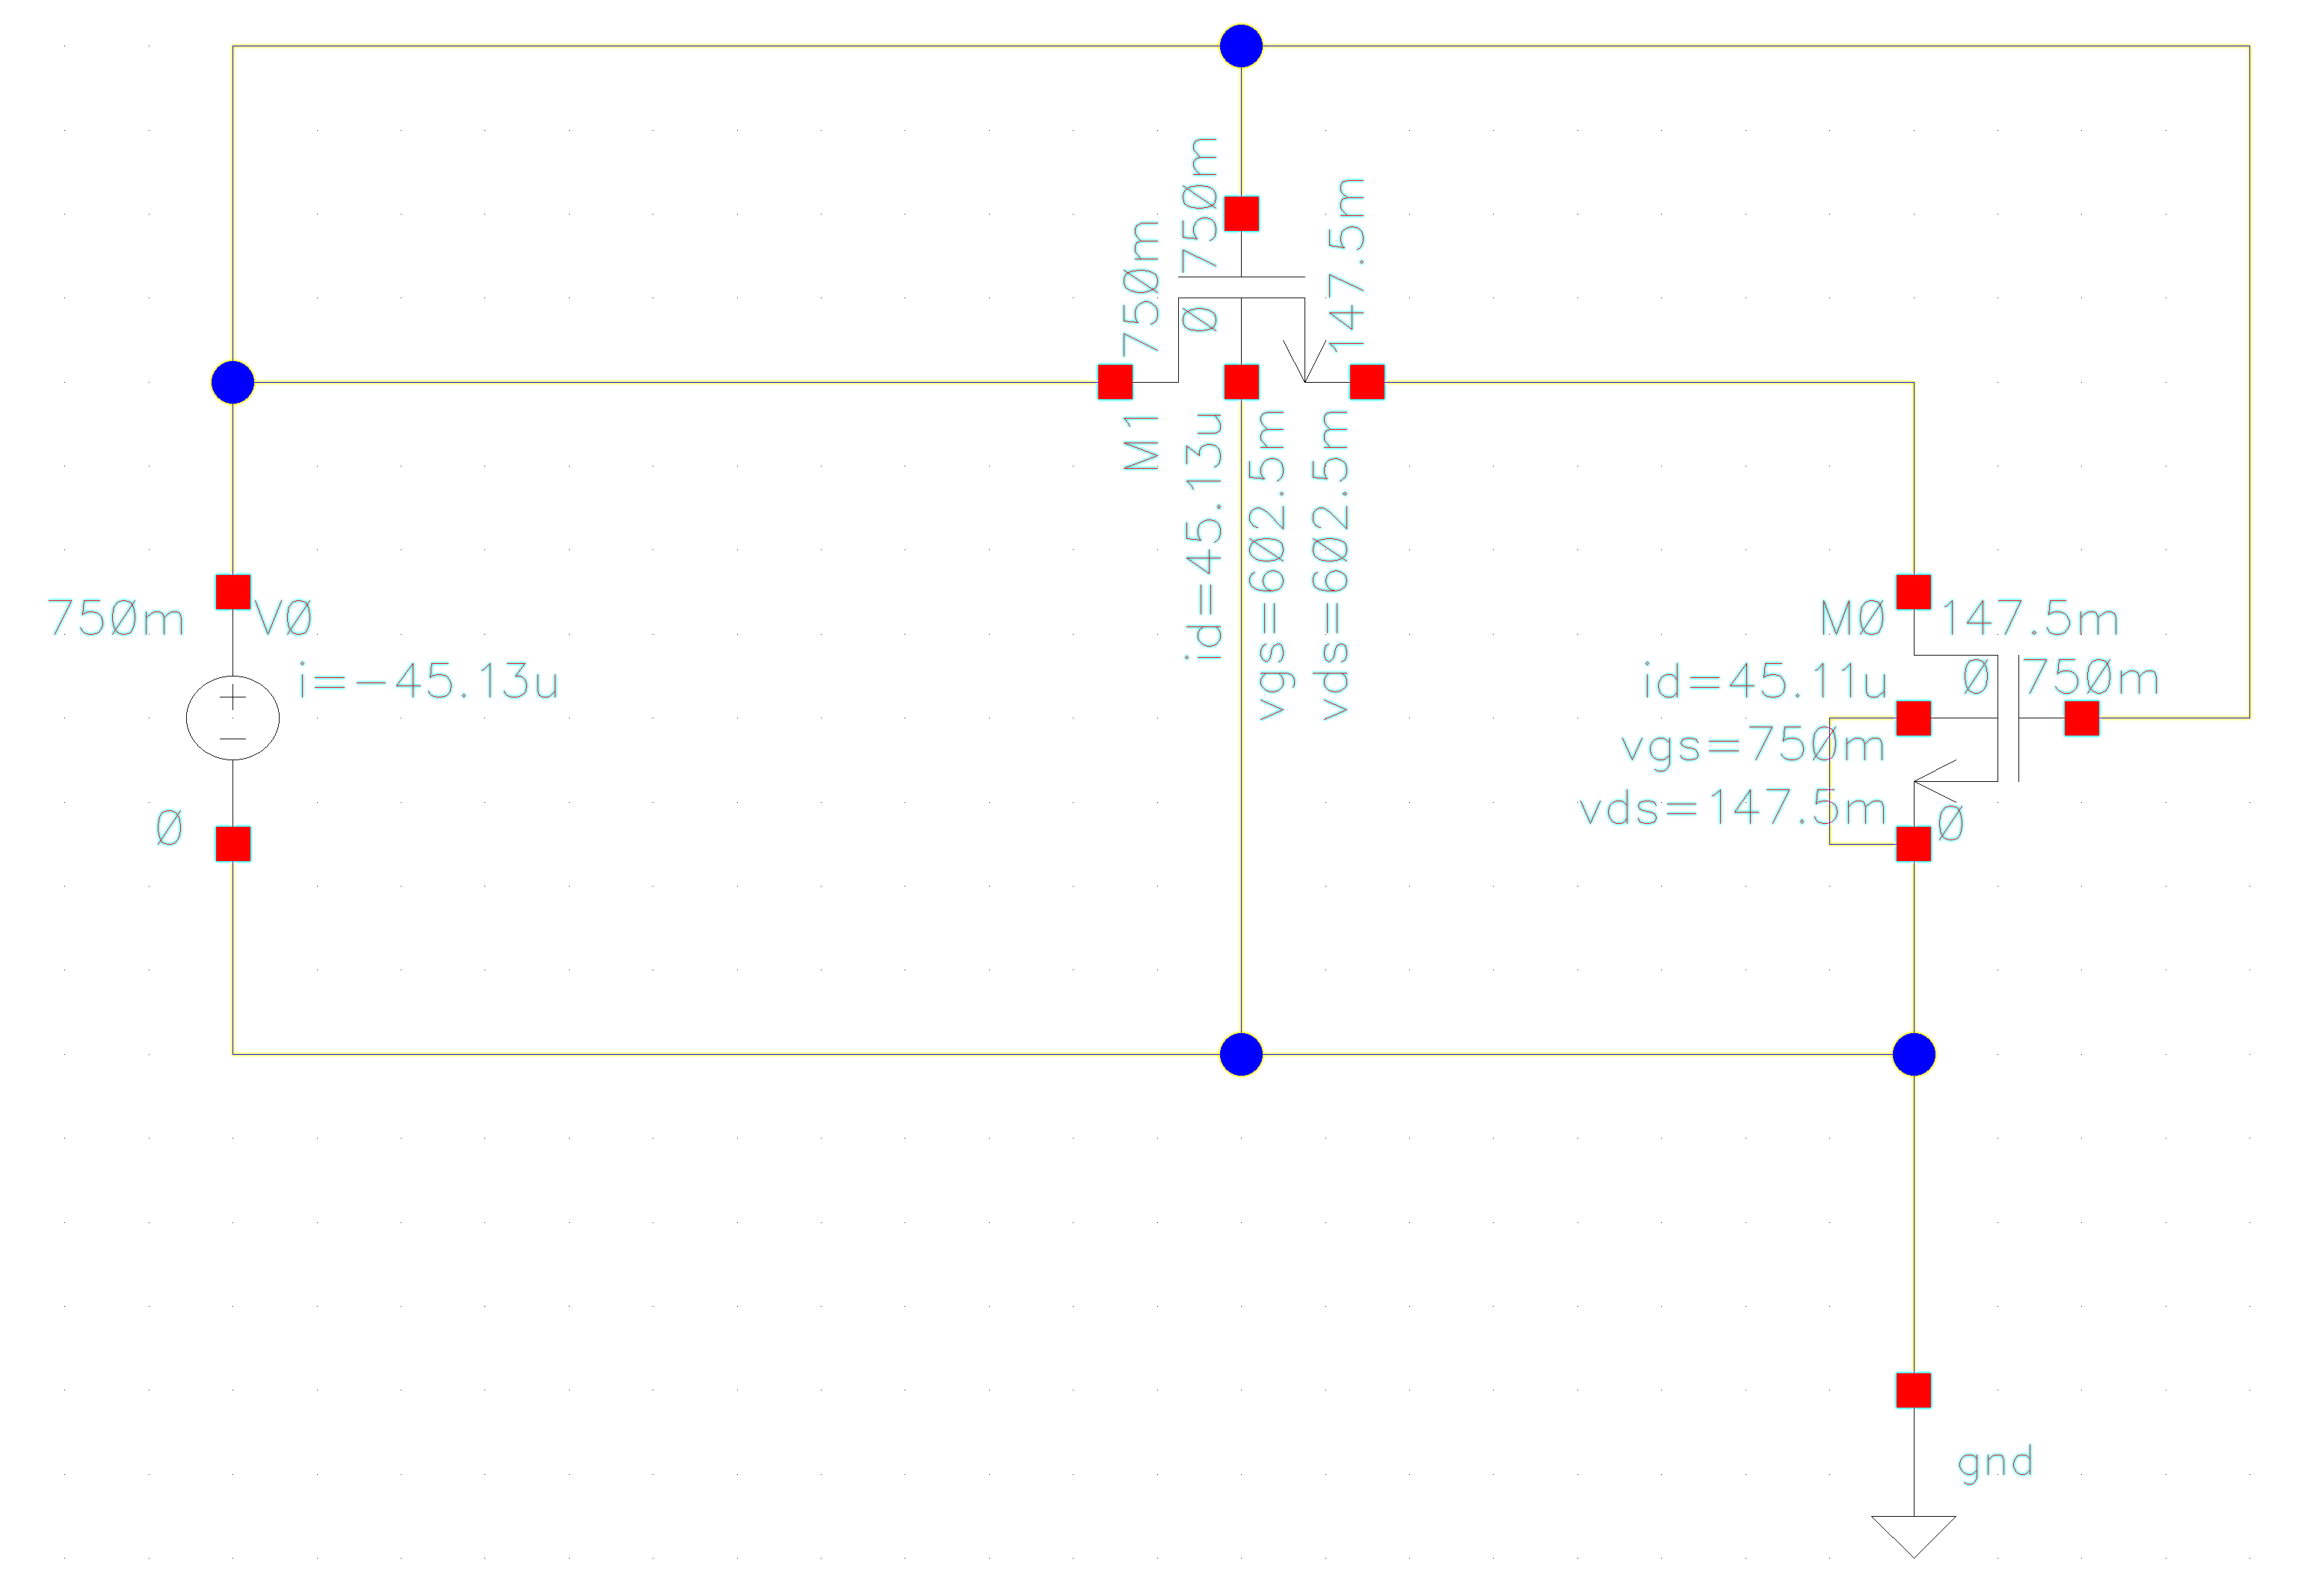
\includegraphics[clip,width=0.45\columnwidth]{Vread-SCHEMATIC.png}
    }
    \subfloat[{Test Circuit for $V_{trip}$}]{
    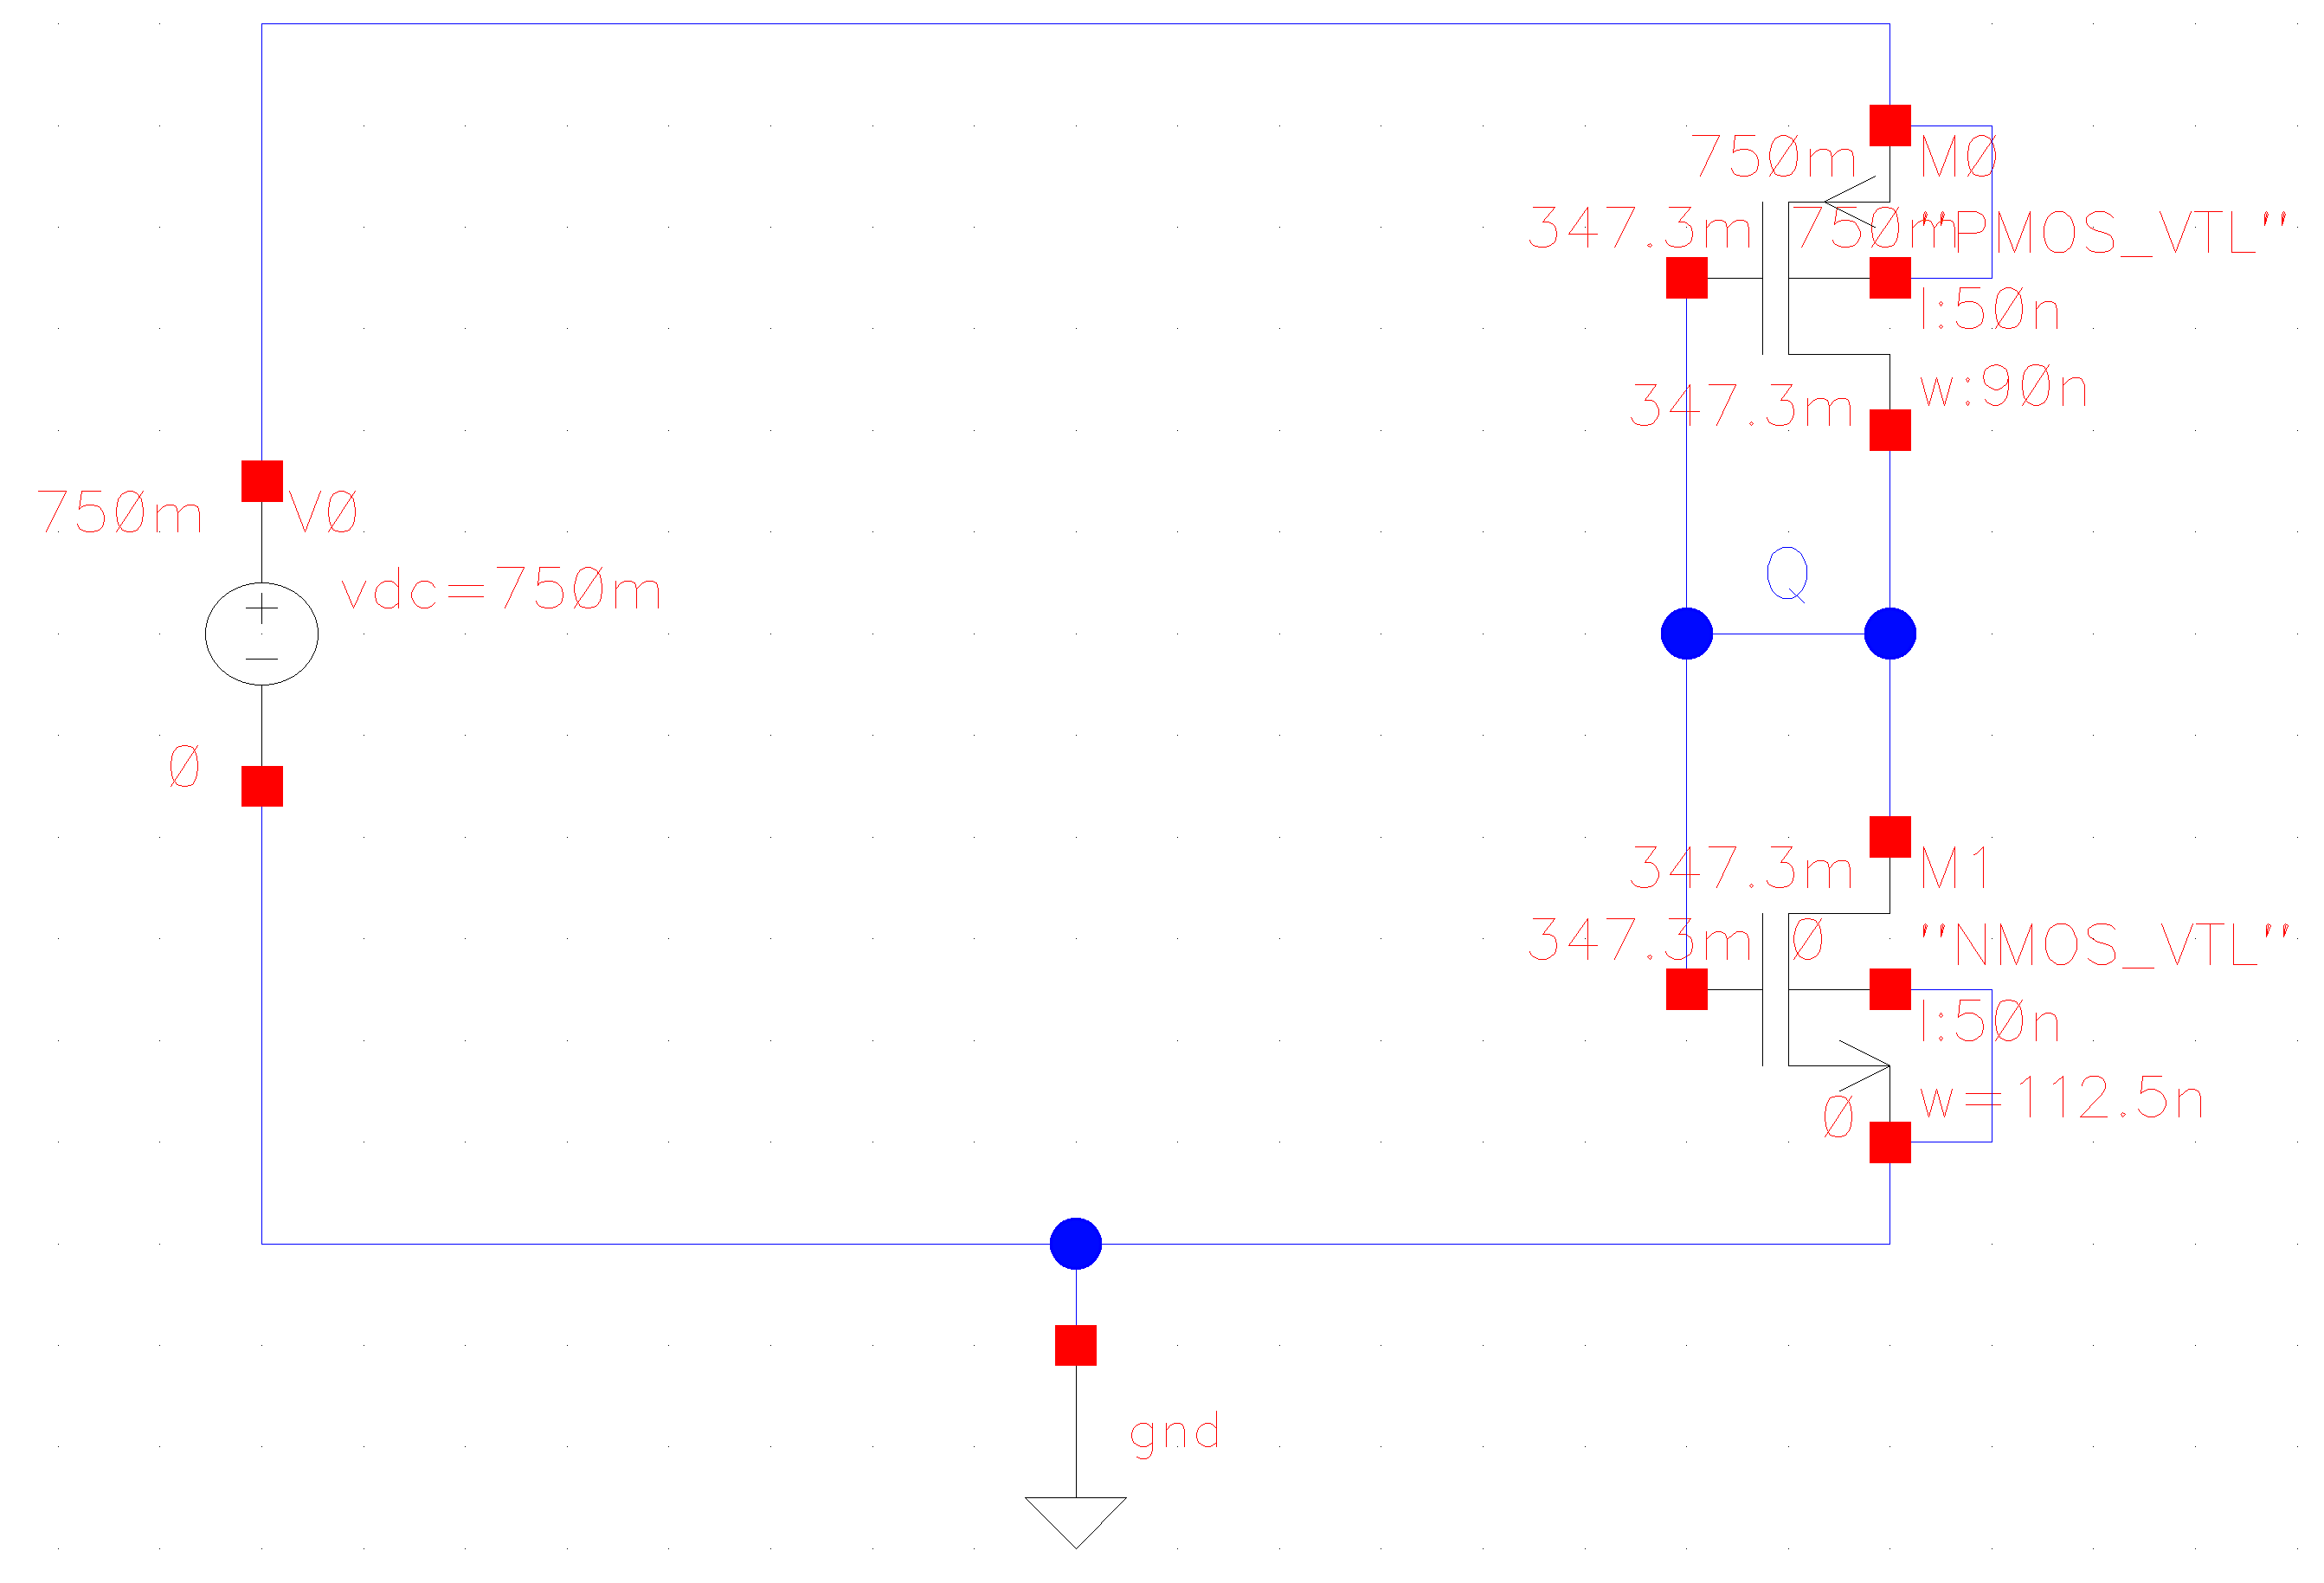
\includegraphics[clip,width=0.45\columnwidth]{Vtrip-SCHEMATIC.png}
    }
    \caption{Test Circuits for Read Noise Margin}
    \label{fig:Vread_Vtrip}
\end{figure}

The DC voltage at the node connecting the access transistor to the pull-down transistor in Figure~\ref{fig:Vread_Vtrip}(a) shows the voltage that Q or QBAR will rise to during a read operation. This voltage should be minimized such that the risk of data destruction is low. The DC current through the two transistors is a factor that affects the cell access time as discussed in section 2. The other contributing factor to this destructive read is the trip voltage of cross-coupled inverters inside the SRAM cell. If the read disturb ($V_{read}$) reaches the trip voltage, then the two inverters will switch to their opposite steady states, thus destroying the stored bit. Figure~\ref{fig:Vread_Vtrip} shows the analysis performed for the optimal sizing described in section 2.3. The read noise margin is then calculated by the equation:
\[ 
  NM_{read} = \frac{V_{trip} - V_{read}}{V_{DD}}\times100\%
\]
\subsubsection*{2. Write Noise Margin Testing}
The determination of the write noise margin is relatively simpler than the calculation of the read noise margin. Figure~\ref{fig:Test_Vwrite} shows the simulation of the scenario where a '0' is being written to the SRAM cell. This operation ideally means [BL] = 0V, and [BL\_BAR] = 750mV. The write margin is a measure of how large the bit line at logic '0' ([BL] in this case), can become before the write operation fails the the data in the SRAM cell doesn't switch.
\begin{figure}[htp]
\centering
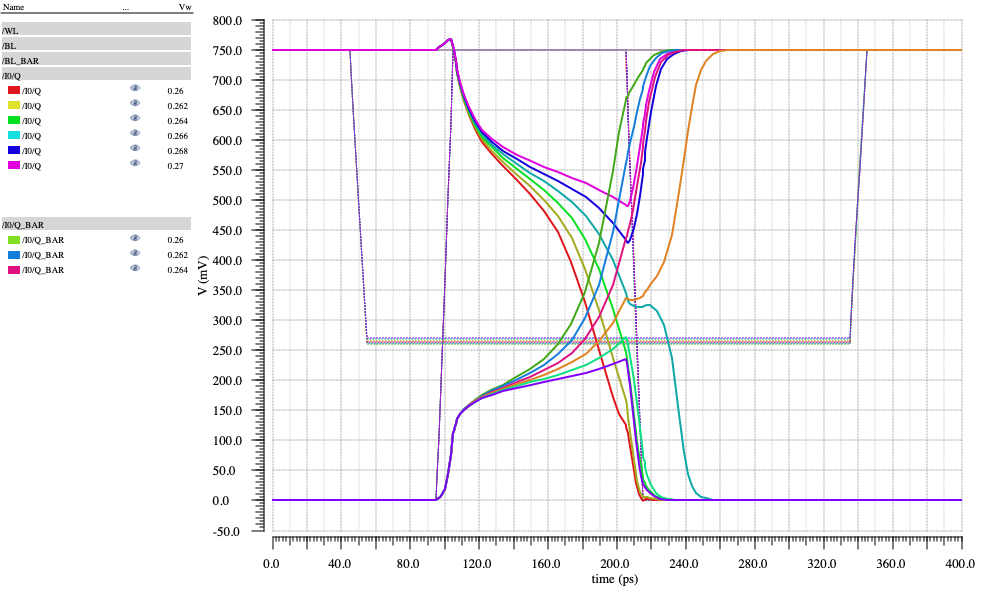
\includegraphics[clip,width=\columnwidth]{Problem2-NM_Write-WAVEFORM.png}
\caption{Parametric Analysis for $V_{write}$}
\label{fig:Test_Vwrite}
\end{figure}
The parametric analysis done in Figure~\ref{fig:Test_Vwrite} sweeps this bit line voltage from 260mV to 270mV and the voltage at which the write operation fails we call $V_{write}$. The write noise margin is then calculated by the equation:
\[ 
  NM_{write} = \frac{V_{write}}{V_{DD}}\times100\%
\]
%\clearpage
\subsubsection*{3. Experimental Sizing Data}
Using the methods described in Appendix A.1 and A.2, the read margin, write margin, and cell access time can be tabulated for all size ratios used in the design process. These values are shown in Table \ref{table:SRAM_test-sizing} below. Note that the data shown in Figures~\ref{fig:NM_Read},~\ref{fig:NM_Write}, and~\ref{fig:Cell_Access} result from plotting the data collected in Table \ref{table:SRAM_test-sizing}.

\begin{table}[htp]
\centering
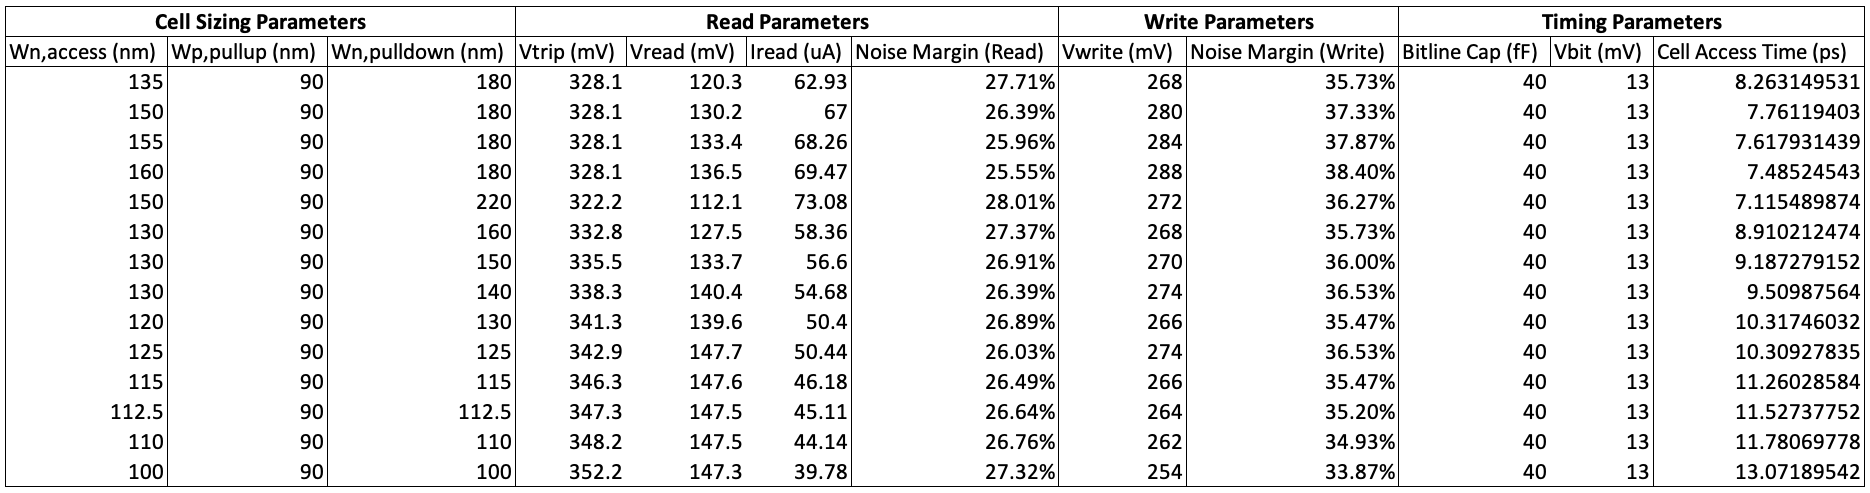
\includegraphics[clip,width=\columnwidth]{Problem2-Table1.png}
\caption{SRAM Experimental Sizing Results}
\label{table:SRAM_test-sizing}
\end{table}

\clearpage
\subsection*{Appendix B}

\subsubsection*{1. Full DRC Report}

\begingroup
\obeylines
\input{SRAM_CELL_DRC_REPORT_2.txt}%
\endgroup%

\subsubsection*{2. Full LVS Report}

\begingroup
\obeylines
\input{SRAM_CELL_LVS_REPORT_2.txt}%
\endgroup%

\end{document}
